\documentclass{article}

% if you need to pass options to natbib, use, e.g.:
%     \PassOptionsToPackage{numbers, compress}{natbib}
% before loading neurips_2020

% ready for submission
% \usepackage{neurips_2020}

% to compile a preprint version, e.g., for submission to arXiv, add add the
% [preprint] option:
%     \usepackage[preprint]{neurips_2020}

% to compile a camera-ready version, add the [final] option, e.g.:
\usepackage[final]{neurips_2020}

% to avoid loading the natbib package, add option nonatbib:
%\usepackage[nonatbib]{neurips_2020}
%{{{ usepackage
\usepackage[utf8]{inputenc} % allow utf-8 input
\usepackage[T1]{fontenc}    % use 8-bit T1 fonts
\usepackage{hyperref}       % hyperlinks
\usepackage{url}            % simple URL typesetting
\usepackage{booktabs}       % professional-quality tables
\usepackage{amsfonts}       % blackboard math symbols
\usepackage{amsmath}       % blackboard math symbols
\usepackage{nicefrac}       % compact symbols for 1/2, etc.
\usepackage{microtype}      % microtypography
\usepackage[]{float}
\usepackage[]{graphicx}
\usepackage{subcaption}
\usepackage[dvipsnames]{xcolor}
%}}}

%{{{ title
\title{Reverse engineering RNN for sentiment classification reveals line attractor dynamics ... and a sling?}

% The \author macro works with any number of authors. There are two commands
% used to separate the names and addresses of multiple authors: \And and \AND.
%
% Using \And between authors leaves it to LaTeX to determine where to break the
% lines. Using \AND forces a line break at that point. So, if LaTeX puts 3 of 4
% authors names on the first line, and the last on the second line, try using
% \AND instead of \And before the third author name.

\author}}
\begin{document}

\maketitle

%{{{ abstract
\begin{abstract} 
  Recurrent Neural Networks (RNN) are widely used to model sequential data such as
  time-series or texts. The can be used for regression (e.g. predicting stock market
  price) or classification (e.g. stock market will increase or decrease).In the 
  original work, the authors explore the dynamic of a trained single-layer RNN 
  for binary sentiment classification (positive versus negative). The authors used tools
  from dynamical system to find fixed points and linearize the nonlinear system around them
  to reveal line attractors with the RNN. In this work, I try to reproduce some of the results
  and improve on mostly studing a 3-layer Gated Recurrent Unit trained on the movie review dataset
  IMDB. We will see that the lower layer is doing grunt work, building the internal 
  representation, and letting the top layer quickly make the decision if a text is 
  positive or negative.
\end{abstract}
%}}}

%{{{ Introduction
\section{Introduction}
The original paper explored 4 types of RNN architectures: LSTM \cite{lstm}, GRU \cite{cho2014learning}, Update Gate RNN \cite{collins2016capacity} and the original flavour of vanilla RNN. Each were trained on three binary sentiment classification dataset: IMDB \cite{IMDB}, polarized movie reviews, Yelp \cite{zhang2015characterlevel}, user reviews, and Stanfort Sentiment Treebank \cite{socher-etal-2013-recursive}, also movie reviews. In each case they trained a single layer. I reached out to the main authors to get their code base, but never got any answer back. So the exact details of the neural architectures are unknown. Did they use dropout? Did they limit the vocabulary in any way? Did they do preprocessing on the texts? There are many details I would have liked to have in order to reproduce as closely as possible their results, but alas I relied on my own experience and what I assume they did. 

To answer the call of the reproducibility challenge, lauched by Joelle Pineau for NeurIPS 2019, I coded everything from scratch\footnote{\url{https://github.com/atremblay/mat6115/blob/master/README.md}} with what little implementation details are available in order to recreate some of the results. If we give ourselves some leaway I believe we can come to the conclusion that the original results are reproducible. 

I focused my efforts on using a GRU trained on the IMDB dataset. My main exploration for this project was to see what kind of dynamic can be observed if we train a two layer GRU instead of just one.
%}}}

%{{{1 Methods
\section{Methods}

%{{{2 Preliminaries
\subsection{Preliminaries}
\label{sec:method-preliminaries}
The n-th RNN cell, GRU in all cases in this work, is denoted as $\textbf{h}_{t+1}^{n}=F^{n}(\textbf{h}_t^{n}, \textbf{x}_t^{n})$ where $\textbf{x}_t$ is the input and  $\textbf{h}_t$ is the hidden state at time $t$. Note that during training $\textbf{x}_t^{n} = \textbf{h}_t^{n-1}$ for  $n > 1$. 

Since we are exploring the dynamics of multi-layers GRU models, the notation $GRU_n$ will refer to the model with $n$ layers.
%}}}2

%{{{2 Training
\subsection{Training}
A very simple, but efficient, model was built. Embedding layer (100 dimensions) -> Dropout(0.5) -> n layers of GRU (256 dimensions)-> Dropout(0.5) -> Fully Connected. The Adam optimizer \footnote{\url{https://pytorch.org/docs/stable/optim.html\#torch.optim.Adam}} with default parameters was used and the loss function is binary cross entropy $Loss=-\frac{1}{N}\sum_{n=1}^{N} y\log\left( \hat{y} \right) + \left( 1-y \right) \log\left( 1-\hat{y} \right)$.

Typical training procedure for machine learning is applied. The dataset is split in train-validation-test sets. Each models are trained, on the train set, for 10 epochs and the parameters giving the lowest loss on the validation are kept for the optimal model.All the analysis in this work are done with the test set only, so the model has never seen those datapoints and no human leakage is seeping through the choice of models. This typically the best, and standard, procedure to get a machine learning model that generalizes as best as possible. I will briefly talk, in the futur direction section (\ref{sec:futur-direction}), how we should perhaps get out of this accepted pattern.

There were no indications in the original paper if all the weights in the networks were learned from scratch or not. Since it is standard practice to use pretrained word embedding I chose to kickstart the learning process with GloVe \cite{pennington2014glove} words vector of 100 dimensions as initial embeddings. Those vectors were trained on a corpus of 6 billion words. "The training objective of GloVe is to learn word vectors such that their dot product equals the logarithm of the words' probability of co-occurrence."\footnote{\url{https://nlp.stanford.edu/projects/glove/}}. Word2Vec \cite{mikolov2013efficient} was also considered, but given that they are often on par and that GloVe was readily available in the library I used I decided to take the path of least resistance. FastText \cite{mikolov2018advances} is also another common choice and quite often seen as a better quality word embedding. Studying the impact of word embeddings is left for futur direction. My educated opinion is that it wouldn't change the observations made here.

Since the author found that their finding is valid for all their dataset I chose to focus on only IMDB movie review dataset. This standard dataset is already split in train-test sets. The train set was subsequently split in train-valid set for the training procedure.
%}}}2

%{{{2 Fixed Point
\subsection{Fixed Point}
\label{sec:method-fixed_point}
Once a recurrent neural network is trained, the inputs become time-dependant parameters while the trained weights are constant over time. The only variable that changes "over time" are the hidden states. That makes it a non-autonomous dynamical system since the function changes its behaviour with time, or in this case as is it "reads" words.
\[
  \mathbf{h}_{t+1} = F\left(\mathbf{h}_t;\pmb{\theta}, \mathbf{x}_t\right)
.\] 

Fixed points are found empirically by minimizing the quantity $q^{n}=\frac{1}{N}\|\mathbf{h}^{n}-F^{n}(\mathbf{h}^{n}, \mathbf{0})\|_2^2$ with respect to the hidden state so we end up at $\mathbf{h}_{*}^{n}=F^{n}(\mathbf{h}_*^{n}, \mathbf{0})$ where $\mathbf{h}_*$ is a hidden state that does not change much under the dynamic of a zero input ($\mathbf{x}=\mathbf{0}$). Using a non-informative constant input has the effect of turning the non-autonomous system into an autonomous one since we get rid of the time-dependant parameters.

The optimization is done by using standard differentiation techniques. If $q$ is less than  $1^{-6}$ then we can consider the hidden state as a fixed point or quasi fixed point. The starting points are 500 hidden states, picked at random, explored by the GRU on the test set (after training). This is done on every layers. If the convergeance of two hidden states bring them to less than $1^{-3}$ in every dimensions then they are considered to have converged to the same point. This is based on the default value of the original fixed point finder code base \footnote{\url{https://github.com/mattgolub/fixed-point-finder}} \cite{Golub2018}.

Some technical difficulties arised. It appears that this cannot be done in bulk but rather one starting point at a time. Unclear if running the optimization in batch create degenerate cases. In other words, every starting point must be run individually and thus we lose the benefits of matrix multiplication acceleration.
%}}}2
%}}}

%{{{1 Results
\section{Dynamics are low dimensional}

Discussion about reproducability of the original paper's result will be threaded in the rest of this report. It's a mix of hit-and-miss, but generally everything holds.

%{{{
\begin{figure}[H]
  \centering
  \begin{subfigure}[b]{0.32\linewidth}
    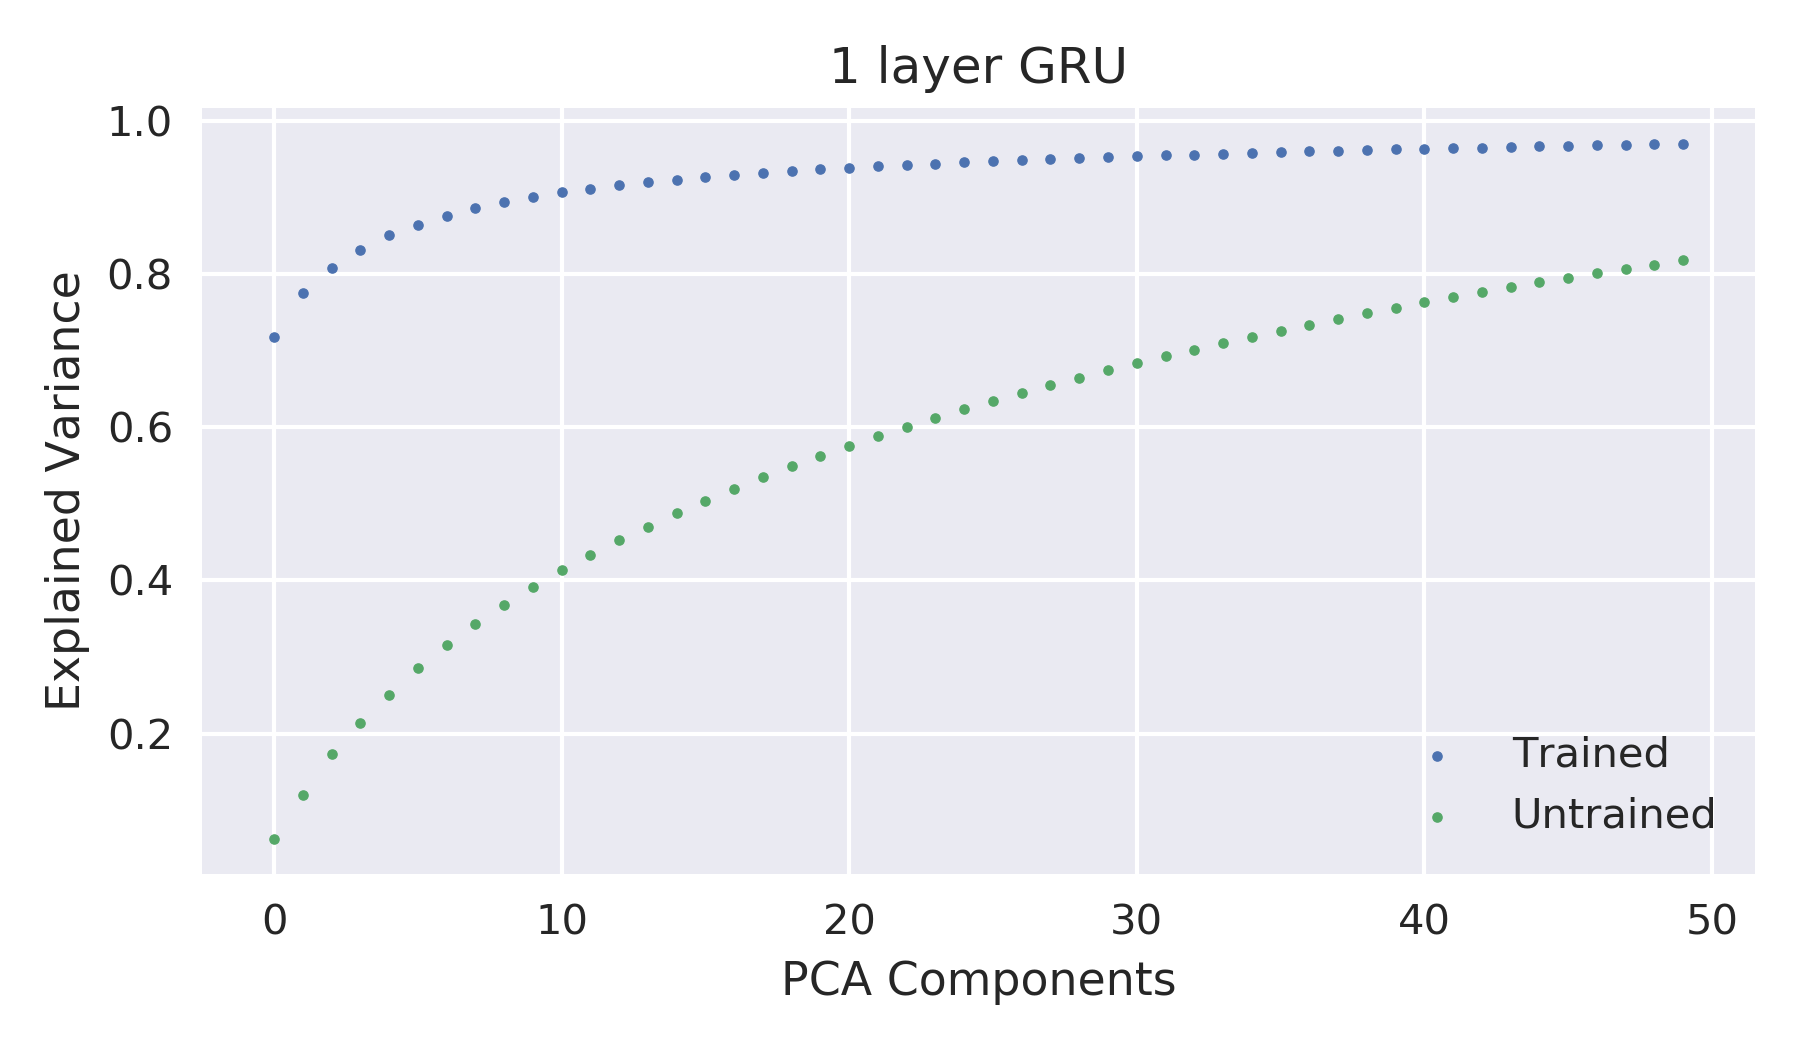
\includegraphics[width=\textwidth]{../images/gru_1layer_100_explained_variance.png}
    \caption{}
    \label{fig:-images-gru_1layer_explained_variance-png}
  \end{subfigure}
  \begin{subfigure}[b]{0.32\linewidth}
    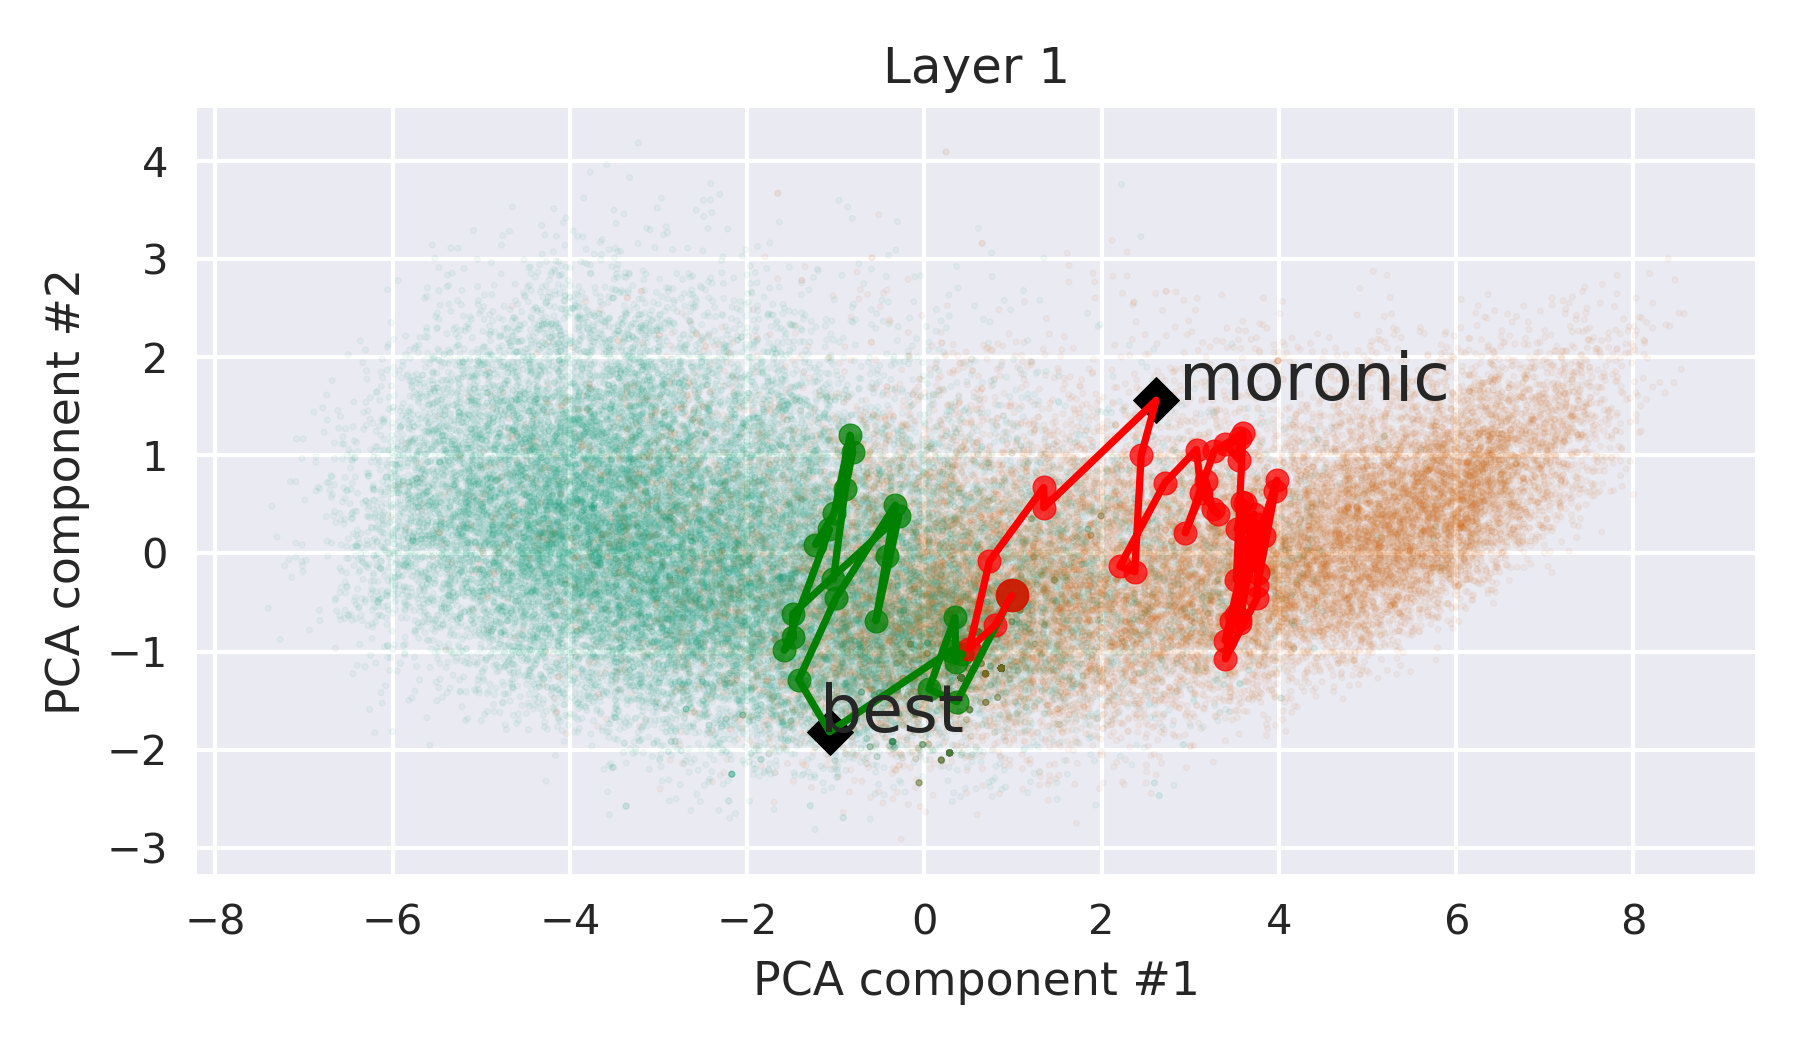
\includegraphics[width=\textwidth]{../images/gru_1layer_100_PCA.png}
    \caption{}
    \label{fig:-images-gru_1layer_PCA-png}
  \end{subfigure}
  \begin{subfigure}[b]{0.32\linewidth}
    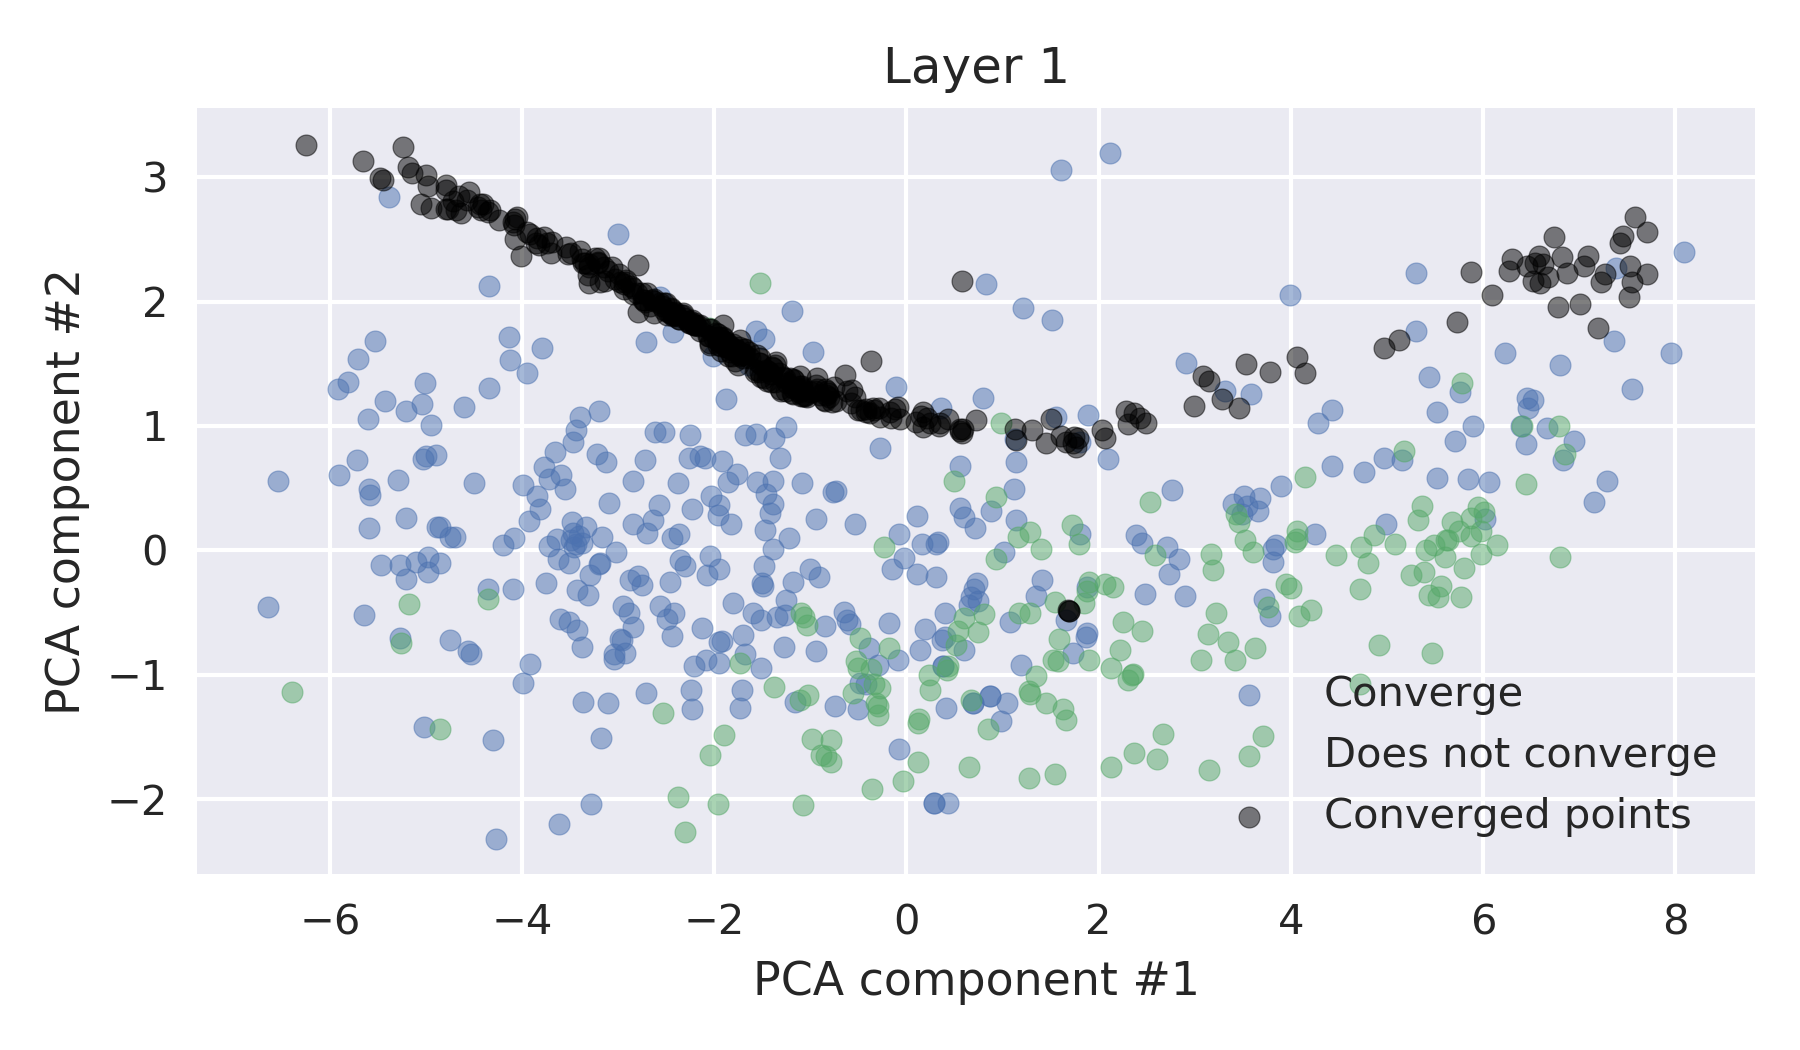
\includegraphics[width=\textwidth]{../images/gru_1layer_100_fixed_points.png}
    \caption{}
    \label{fig:-images-gru_1layer_fixed_points-png}
  \end{subfigure}
  \caption{
    (\ref{fig:-images-gru_1layer_explained_variance-png})
    Explained Variance for a trained 1 layer GRU on IMDB versus untrained. 
    The first few dimensions rapidly explain 90\% of the variance. Only the first 50 dimensions are shown.  
    (\ref{fig:-images-gru_1layer_PCA-png})
    First 2 PCA components on the 1 layer model colored by labels. The evolution of the 
    hidden state of a positive and negative examples are overlayed.
    (\ref{fig:-images-gru_1layer_fixed_points-png})
    500 hidden states sampled and updated until convergeance as described in (\ref{sec:method-fixed_point}).
  }
\end{figure}
%}}}

%{{{2 PCA
\subsection{PCA}

Even though the hidden states of the GRU cells are 256 dimensions, most of the action, once the model is trained, is happening in much less dimensions.

In order to observe the low dimensionality of the dynamics, a PCA is trained on all the hidden states visited by the model on the test set. A 1-layer GRU, $GRU_1$, trained on the polarity task quickly learns to embed all the relevant information in very few dimensions, as can be seen in (\ref{fig:-images-gru_1layer_explained_variance-png}). It takes only the first few PCA components to explain 80-90\% of the variance. An untrained GRU cell contains, as expected, very little information and requires many more dimensions to reach the same level of explained variance. We will see later how having only 1 layer forces the network's hand. This result is somewhat similar to the original paper (\cite{maheswaranathan2019reverse} - figure 12).

\begin{figure}[H]
  \centering
  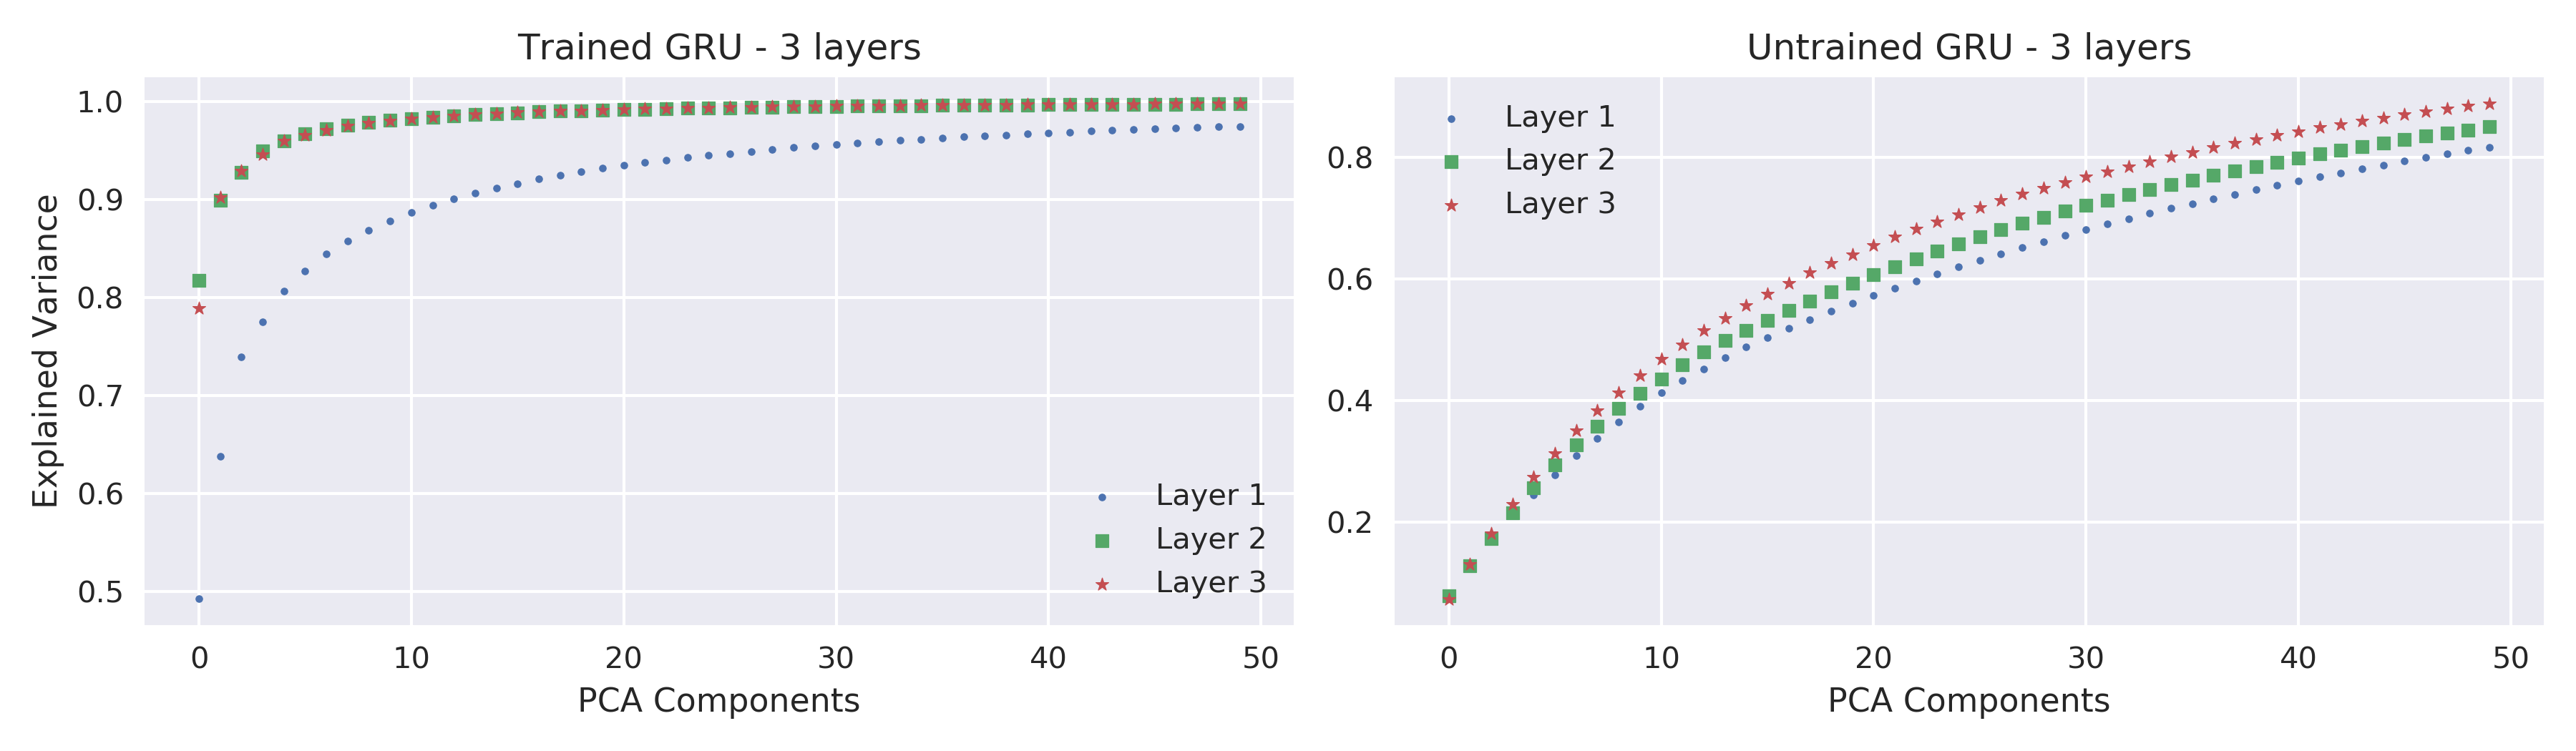
\includegraphics[width=1\textwidth]{../images/gru_3layer_100_explained_variance.png}
  \caption{Explained Variance for a trained 3 layer GRU on IMDB versus untrained. 
    Contrary to the 1 layer model, the first layer requires many more dimensions 
    to explain the same variance. The second and third layer requires much less dimension 
    to explain the same level of variance compared to the 1 layer model. Only the first 50 dimensions are shown.
  }
  \label{fig:-images-gru_3layer_explained_variance-png}
\end{figure}

Similar to the 1-layer case, a PCA was trained on the hidden states visited by each GRU layers on the test set. In other words, we have as many PCA as there are layers, they are trained independantly as they do not encode the same information and do not live in the same space (figure \ref{fig:-images-gru_3layer_PCA-png}).

Unlike the explained variance of $GRU_1$, the first layer in this model requires much more dimensions to explain the same variance when considering the PCA components. After the first 50 dimensions we reach about the same level of explained variance. The biggest difference can be seen in the first 2 components where the 1-layer model explains close to 80\% while the first layer of the 3-GRU barely explains 60\%. 

The second and third layer on the other hand encode all the relevant information in even less dimensions than the 1-layer model. The first 2 components explain over 90\%. A possible explanation would be that the 1-layer is doing all the grunt work, weeding out the grass so that the subsequent layer can focus on the relevant information, similar to a CEO getting all the distilled informations from the lower management. 

In a way, the PCA on $GRU_1$ shows that the model is forced to learn very rapidely and encode everything in its limited capacity. By itself it is not obvious why having less capacity would force the model to encode the task in as little dimensions as possible whereas the first layer of $GRU_3$ has more leeway. This is a mystery to me. In fact, before working on this assignment I thought that the network fully made use of the space given to it.
%}}}2

%{{{2 Projections
\subsection{Projections}

Figures \ref{fig:-images-gru_1layer_PCA-png} and \ref{fig:-images-gru_3layer_PCA-png} show the projection on the first 2 PCA components of the visited hidden states of the test set by $GRU_1$ and $GRU_3$ models respectively. The points are colored by their corresponding labels. Additionnally, to help wrap our head around the dynamic, we look at the evolution of the hidden states of two movie reviews. Both reviews are run through $GRU_n$ and the positive hidden states $\left\{\mathbf{h}_1^+, \mathbf{h}_2^+, \ldots \mathbf{h}_p^+\right\}$ and negative hidden states $\left\{\mathbf{h}_1^-, \mathbf{h}_2^-, \ldots \mathbf{h}_n^-\right\}$, at every layers, are projected on the first 2 PCA components.

Positive
\begin{flushleft}
\hbox{%
  {\color{ForestGreen}\vrule}\hspace{.5em}\parbox{.9\textwidth}%
{It is by far one of the best comic book adaptations ever. I liked this one even more than X-men.}
}
\end{flushleft}

And negative

\begin{flushleft}
\hbox{%
{\color{red}\vrule}\hspace{.5em}\parbox{.9\textwidth}%
{  First of all I hate those moronic rappers, who couldn't act if they had a gun pressed against their foreheads. All they do is curse and shoot each other and acting like cliché'e version of gangsters.
}
}
\end{flushleft}
Figure (\ref{fig:-images-gru_1layer_PCA-png}) is a reproduction of the original results (see \cite{maheswaranathan2019reverse} - figure 12). The itinial starting hidden state (where the two path starts) is slightly different than the original paper, but this difference may very well be explained by the differences in training or even the random initialization of the network. Considering how the two examples evolve in this 2-dimension projection, we can see that they stay close to the middle at the beginning when the words are non-informative. Once the emotionally charged words \textit{best} and \textit{moronic} are "read", then the hidden states go their separate ways and then keep more or less stumbling around. They are likely moving in higher dimensions and what we see here is a project so us mere mortal can visualize it. 

\begin{figure}[H]
  \centering
  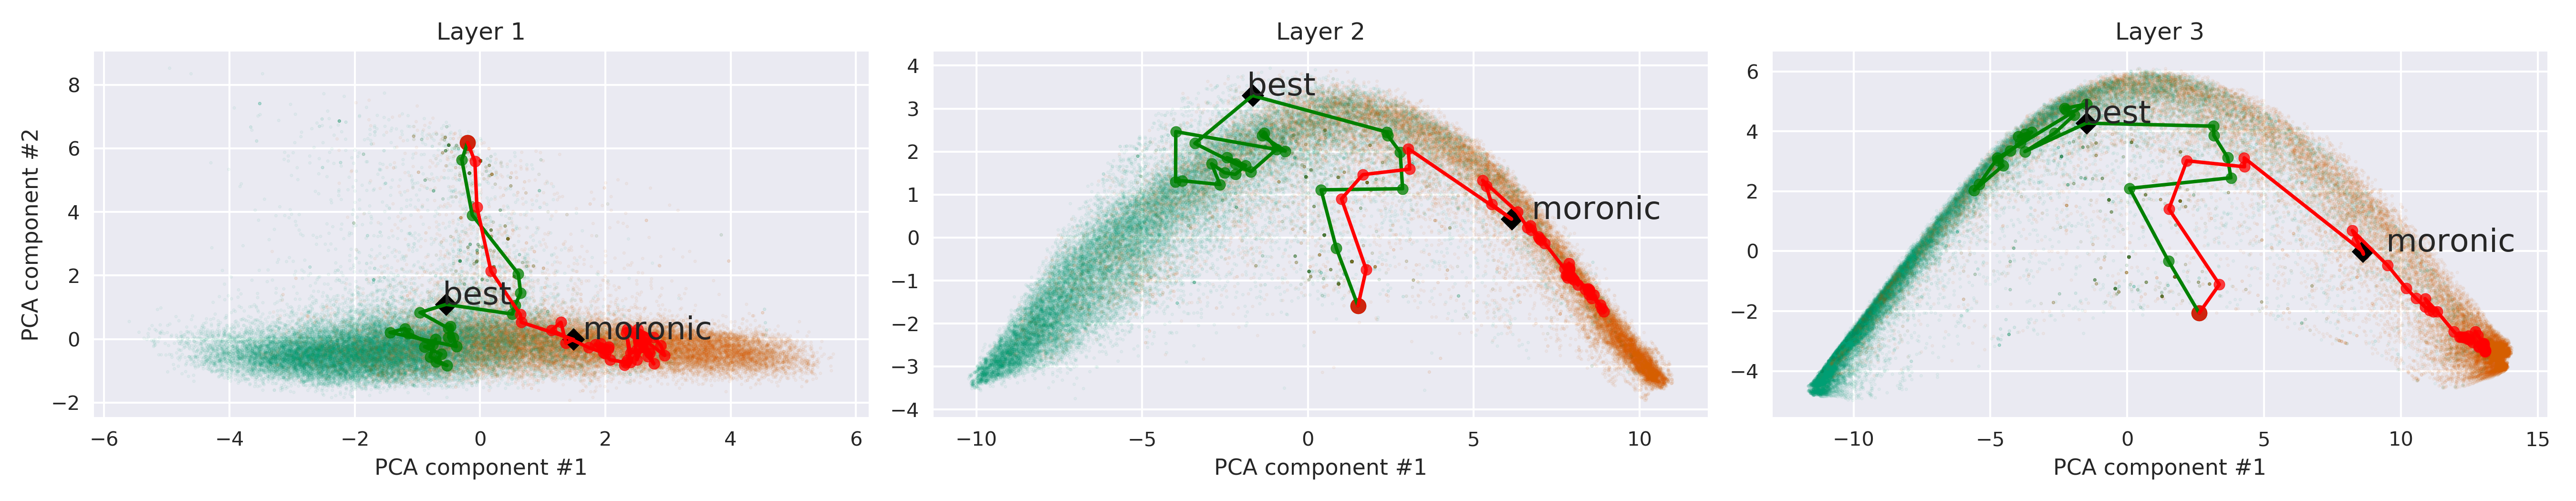
\includegraphics[width=1\textwidth]{../images/gru_3layer_100_PCA.png}
  \caption{
    First 2 PCA components on each of the 3 layer model, colored by labels. 
    The evolution of the hidden state of a positive and negative example are overlayed.
  }
  \label{fig:-images-gru_3layer_PCA-png}
\end{figure}  

Now comes the interesting part. Visualizing the first two PCA components of each layers of $GRU_3$ (figure \ref{fig:-images-gru_3layer_PCA-png}) starts revealing interesting behaviours. Let's focus our attention to the evolution of the hidden states of the positive and negative examples. For the first layer, considering that the first two PCA components does not explain a whole lot of the variance, the path taken by the examples seems to be stumbling around. The activity is not as low dimensinal as in the 1-layer case.

The second and third layers have activity in much lower dimensions, even lower than the 1-layer case. The evolution of the examples are less stumbling around, more to the point for the task it was trained on. 

An analogy that comes to mind is that the 1-layer model is like the undergrad student focusing on a higher understanding to get good enough grades and a good job. The 3-layer model is like a PhD that spent a lot of time to master the foundations of his field (first layer) and focused on his area of research during his graduate years (second and third layers). That student has a larger understanding of the foundation and when it comes to his specialization it's like a sharp shooter. 

It may be strange that the starting points are far from the rest of the hidden points, but it makes total sense. Just like it makes no sense to go to the driving range and practice only your wood 1, there is far less starting shot in golf than approach shots, it makes no sense to expect starting points to be close to the rest because there are far less initial words than in-sentence words. Another interesting observation is the impact of emotionally charged words. In the positive example, the result of "reading" the word \textit{best} results in a sudden change in the hidden state in every layer. It's even more apparent in the top layers. Similarly, the word \textit{moronic} makes the negative example shoot to the right, towards the negative area, very rapidely. It may be oversimplistic, but if we consider the first component to encode the task at hand, namely sentiment analysis, then the change of direction in that dimension could be used as low-tech explanation for the impact of the word. This may be an unwarranted simplification as this explanation could very well be overfitting these particular observations.
%}}}2

%{{{2 Fixed Points
\subsection{Fixed Points}
\label{subsec:fixed-points}

In (\ref{fig:-images-gru_1layer_fixed_points-png}) we can see where the fixed point procedure (\ref{sec:method-fixed_point}) ends up. 500 hidden states were sampled and ran until convergeance. Recall that the fixed point procedure uses a constant input vector $\textbf{0}$ whereas all the hidden states present are actual hidden states from real text.

And now for the crux of the conversation we look at the fixed points. As described in the preliminaries \ref{sec:method-fixed_point}, fixed point are found by minimizing the quantity $q^{n}=\frac{1}{N}\|\textbf{h}^{n}-F^{n}(\textbf{h}^{n}, \textbf{0})\|_2^2$ at every layer $n$ where  $\textbf{h}^n$ is the hidden state going in at the n-th layer with a constant input of zero. Iteratively the starting hidden state is modified through gradient descent until it stabilizes (until $q < 1e-6$). If it never reaches that threshold then the starting hidden state is said to not converge. Figure \ref{fig:-images-gru_3layer_fixed_points-png} shows the start of 500 hidden states selected at random; the blue ones are points that ultimately converge and the green points don't. The black dots are where the convergeance ends. Two hidden states are converging to the same point if they end up in a hypercube of side $1^{-3}$ \footnote{Taken directly from the default value of the original paper}.
\begin{figure}[H]
  \centering
  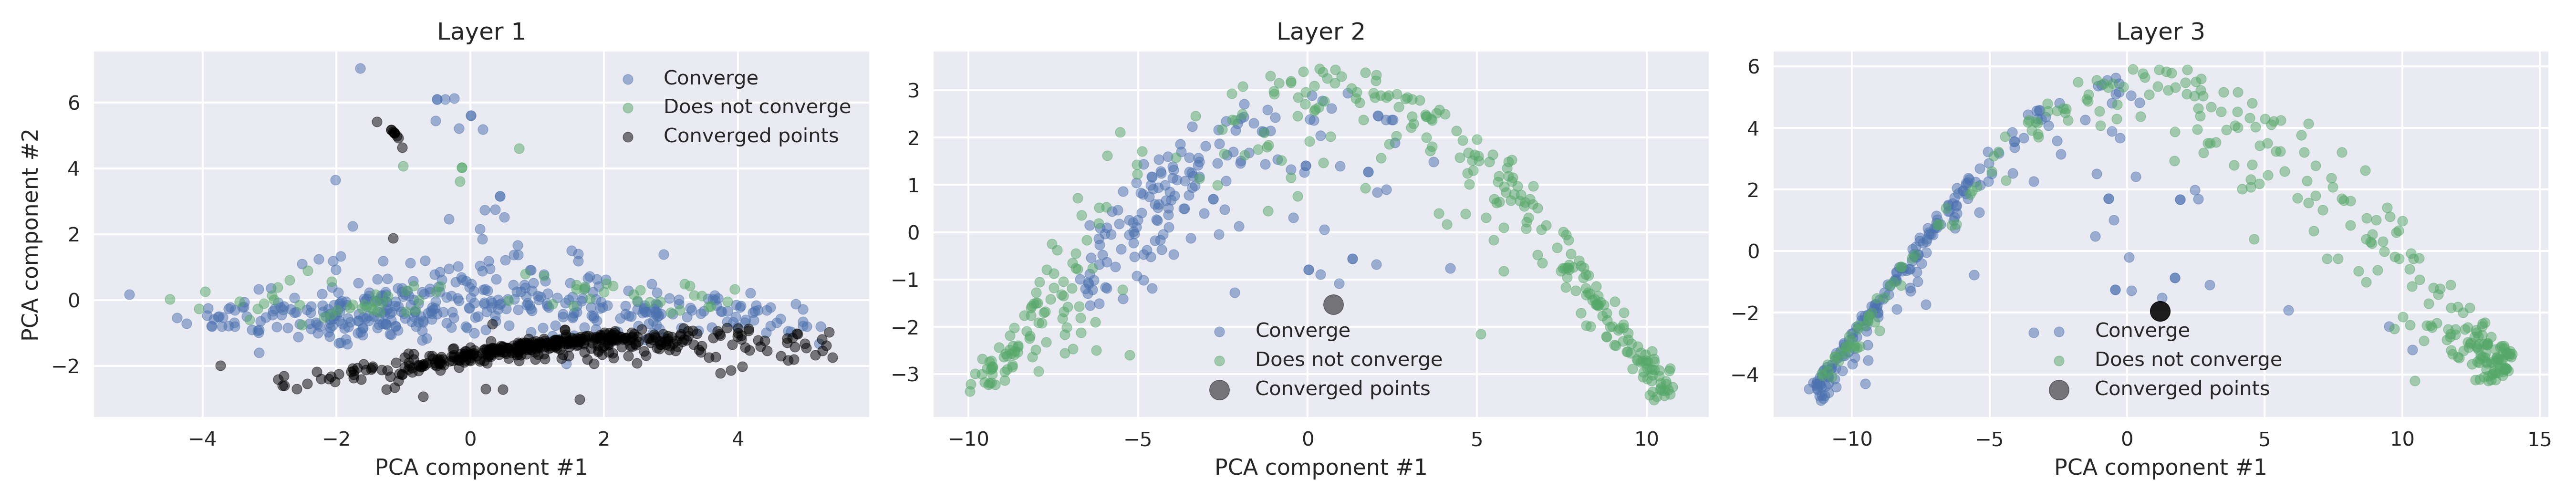
\includegraphics[width=1\textwidth]{../images/gru_3layer_fixed_points.png}
  \caption{Fixed points for 2 layer GRU}
  \label{fig:-images-gru_3layer_fixed_points-png}
\end{figure}
The first layer has many of these fixed points and interestingly they are close to the projection of the initial hidden states. Whereas the second has only one and the third has three (they are so close they could be considered the same but are not due to the condition described above). Here we can observe a different behaviour, the rare fixed points are far from the rest of the points, standing suspiciously in the middle of the horse shoe. We will discuss this in the Fixed Point section below (\ref{subsec:fixed-points}). One could think that there is a bug in the code, but considering that similar results as the orignal paper are reproduced (see figure \ref{fig:-images-gru_1layer_fixed_points-png}) then we can move forward with the analysis. Looking at the evolution of the hidden states of the positive and negative examples in the PCA space (figure \ref{fig:-images-gru_3layer_PCA-png}) was already hinting at these fixed points and their linearization.
%}}}2

%{{{2 Linearization
\subsection{Linearization}

The linearization around the fixed point of a GRU is, not surprisingly, done with a Taylor expansion

\begin{align}
  \textbf{h}_t^n &= F\left( \textbf{h}_*^n + \Delta \textbf{h}_{t-1}^n, \textbf{x}_*^n + \Delta \textbf{x}_{t-1}^n \right) \\
                 & \approx F\left( \textbf{h}_*^n, \textbf{x}_*^n \right) + \textbf{J}_n^{rec}\Delta \textbf{h}_{t-1}^n + \textbf{J}_n^{inp}\Delta \textbf{x}_{t-1}^n
\end{align}

Where $\Delta \textbf{h}_{t-1} = \textbf{h}_{t-1} - \textbf{h}_*$, $\Delta \textbf{x}_{t-1} = \textbf{x}_{t-1} - \textbf{x}_*$ and $\left(\textbf{J}^{rec}, \textbf{J}^{inp}\right)$ are the Jacobian matrices  of the system:  $J_{ij}^{rec}=\frac{\partial F\left( \textbf{h}^*, \textbf{x}^* \right)_i }{\partial h^*_j} $ and $J_{ij}^{inp}=\frac{\partial F\left( \textbf{h}^*, \textbf{x}^* \right)_i }{\partial x^*_j} $. To not overload the notation the indices denoting the $n^{th}$ layer is not always shown. I trust my dear reader will be able to follow. A star always denote the fixed point, whether it's in subscript or superscript.\\
$\textbf{h}_*$ is found numerically and  $\textbf{x}_*=\textbf{0}$. Using those fixed points the linearization reduces to
\[
  \Delta \textbf{h}_t = \textbf{J}^{rec} \Delta \textbf{h}_{t-1} + \textbf{J}^{inp}  \Delta \textbf{x}_{t}
.\] 

Obviously the linearization depends on which hidden states we start from and we can see, in both figures \ref{fig:-images-gru_1layer_eig-png} and \ref{fig:-images-gru_3layer_eig-png}, up to three different sets of eigenvalues of the Jacobian $\textbf{J}^{rec}$ of the linearization around fixed points, for every layers.

\begin{figure}[H]
  \centering
  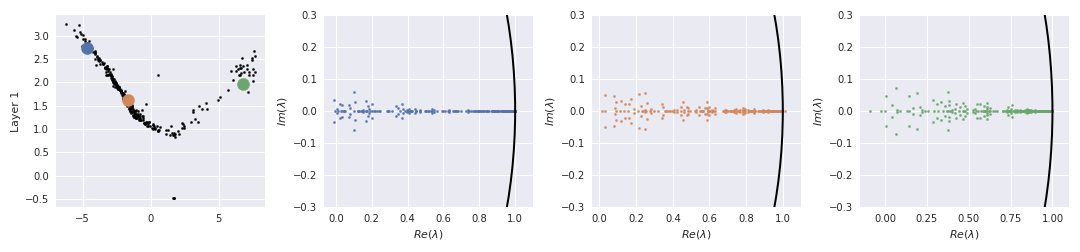
\includegraphics[width=1\textwidth]{../images/gru_1layer_100_eig.png}
  \caption{Eigenvalues of the linearization around different fixed points for the 1-layer model.
  The unit circle is show in black.}
  \label{fig:-images-gru_1layer_eig-png}
\end{figure}

This is where the results diverge the most from the original paper. No direct comparison can be done since they only show this part for an LSTM model trained on the Yelp dataset. Based on the description of their results, I was expecting to find quite similar results for GRU trained on IMDB. Alas, this is not exactly the case. In their figure 3b (\cite{maheswaranathan2019reverse}) there are almost no visible imaginary part for their eigenvalues. Or perhaps it's a plotting defect and they are simply not visible enough. Regardless, figure \ref{fig:-images-gru_1layer_eig-png} shows the eigenvalues of the linearization around three different fixed points. 

The conclusion of the autors was that across the range of fixed points, the eigenvalues are mostly real (no imaginary part) and less than 1. We can still observe the same behaviour, but not to the same extent. There are many more eigenvalues with imaginary part with positive real parts then what they are getting. The imaginary parts are closer to the origin, so this shows a slow expanding rotation in some dimensions while the eigen values without imaginary parts are close to 1 on the real axis. This is turns show an attraction.

\begin{figure}[h]
  \centering
  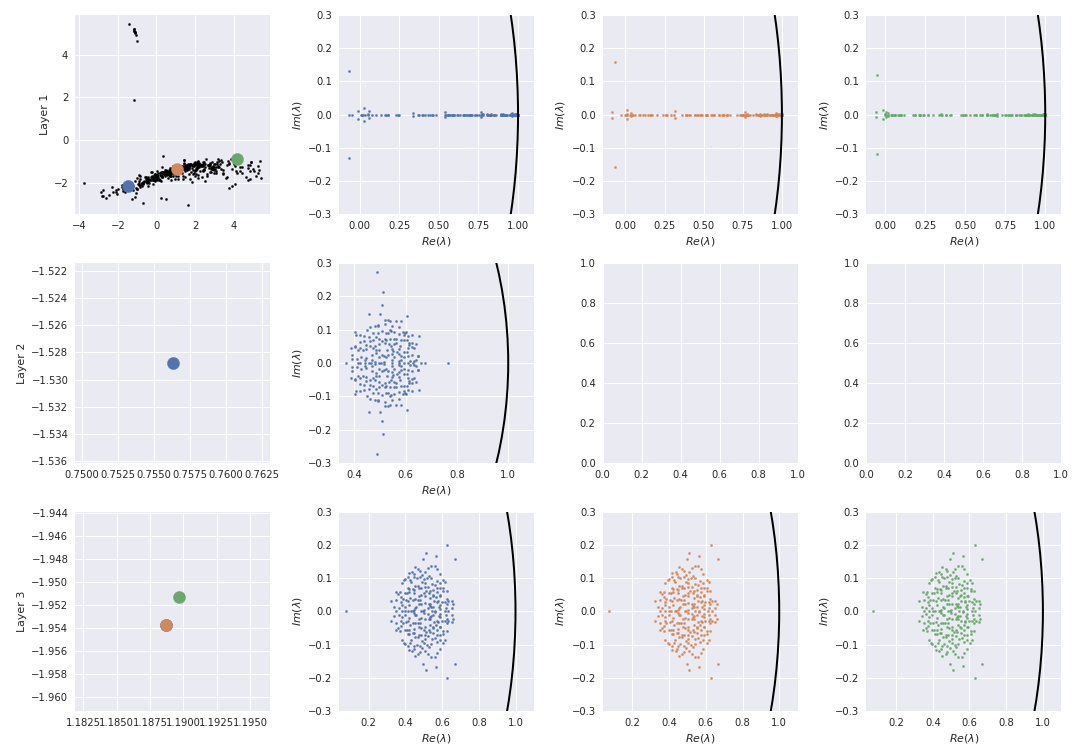
\includegraphics[width=1\textwidth]{../images/gru_3layer_100_eig.png}
  \caption{Eigenvalues of the linearization around different fixed points for the 3-layer model.
  The unit circle is shown in black.}
  \label{fig:-images-gru_3layer_eig-png}
\end{figure}

And the fascinating cherry on top of the proverbial sunday is finally here. In the layer 1 of figure \ref{fig:-images-gru_3layer_PCA-png} we see the starting point of the positive and negative examples far from the point cloud only to converge to that cloud as words are input. Looking at the eigen values of the Jacobian $\textbf{J}^{rec}$ for three different hidden states, a similar line attractor as described in the original paper appears. Most of the eigen values have no imaginary part, thus no rotation, and real parts less than one. This means that there is convergeance and because every hidden states are showing similar behaviour we can empirically conclude that there is a line attractor. As mentioned above, the fixed points are basically in the cloud of hidden states.

The fixed points of the second and third layers are very different. Again, the starting hidden states are far from the cloud and get there as words are read, as if they were repelled from the fixed point. Looking at the eigen values of the Jacobian of the recurrent input ($\textbf{J}^{rec}$) reveals almost exclusively rotations going away from the fixed point (i.e. eigen values with imaginary parts and positve real parts). It's as if the first layer did all the grunt work and the top layers are all amped up and ready to run. They're running circles around their starting block and waiting for their signal. Building on the first layer's work, they are ready to jump to conclusion.
%}}}2
%}}}1

%{{{1 Discussion
\section{Discussion}

The above results are a bit difficult to generalize. We must take a brief look at the 2-layer (\ref{anx:2-layers}) and 4-layer (\ref{anx:4-layers}) cases.

\subsection{2 layers GRU}
The explained variance of the PCA components somewhat follows the same pattern as in the 3-layer model. That is, the first layer is not as low dimensional as the second one, but it also requires three times more components than the first layer of $GRU_3$ or even the $GRU_1$. Second layer still requires very few dimensions.

The 2D PCA projection (\ref{fig:-images-gru_2layer_PCA-png}) is also different than $GRU_3$. The positive and negative examples start right in the middle of the projection rather than slightly outside. In itself I don't think it's that much of a deal. It's simply odd that it looks more like two $GRU_1$ stacked on top of each other compared to $GRU_3$. This observation is solidifed when we look at the fixed point (\ref{fig:-images-gru_2layer_fixed_points-png}). Compared to $GRU_3$ I was expecting the second layer to have a single (or very few) fixed point in the middle of a horse shoe, but instead we see another line attraction. Based on the eigenvalues (\ref{fig:-images-gru_2layer_eig-png}), the second layer is even more a line attractor than the first one.

\subsection{4 layers GRU}
Similar observation can be made for $GRU_4$. First layer requires 3 times as many dimensions to explain 90\% compared to $GRU_1$ and $GRU_3$. It would be natural to expect, based on what we have seen so far, that every layer would be lower and lower dimensional, but the $4^{th}$ is slightly higher dimensional than the $3^{rd}$ one.

The 2D PCA projections (\ref{fig:-images-gru_4layer_PCA-png}) is, again, different. Based on what we have seen so far it's difficult to find a pattern of what to expect and when. The second and third layers looks almost similar while something seems to be going wrong in the fourth layer. It looks like a pile of sand blasted away. But in all cases, we can still see the impact of emotionally charged words (\textit{best} and \textit{moronic}). They are a key differenciator.

If, based on $GRU_3$ we were expecting to find single fixed points in every layer but the first one we would be wrong. Second and third layers do have a single (of very very few) fixed points, but the fourth layer is showing an evey stronger line attractor than anything we have seen so far. At this point I think it has something to do with overfitting. 4 layers for this task is pushing it.

\subsection{3 layers GRU with embedding of 50 dimensions}
To reinforce the idea that there is no discernable pattern, figures \ref{fig:-images-gru_3layer_50_explained_variance-png}, \ref{fig:-images-gru_3layer_50_PCA-png}, \ref{fig:-images-gru_3layer_50_fixed_points-png} and \ref{fig:-images-gru_3layer_50_eig-png} show the dynamics of a $GRU_3$ with an embedding of 50 dimensions instead of 100. Layer 2 is showing similar dynamics as the $GRU_3$ with an embedding of 100 dimensions, but the first and last layers are completely different. They are almost flipped (no bug in my code), the attractor is at the very end. This is fascinating. Under the non-informative input ($\mathbf{X} = \mathbf{0}$) the last layer is essentially being conservative and attracts the hidden state. Perhaps they are a bunch of local minima.

%}}}1

%{{{1 Futur direction
\section{Futur direction}
\label{sec:futur-direction}

As previously mentioned, using the first PCA component to try and explain the impact of each word may be too simplistic. We could convince ourselves, perhaps on a case-by-case basis, that this is a reasonable thing to do. At the very least, more empirical observation could be made on binary task such as predicting bear/bull position for stock market or even multiclass problems where we cannot simply split the plane in half.

Analyzing the behaviour of an RNN this way may push the boundaries in interpretability of deep learning. I am often asked why an NLP makes its prediction, why an obviously easy example (for a human) gets misclassified. It would be enlightening, from a business perspective, to be able to explain some of the decisions of the model to machine learning moguls. In my experience, I typically managed to calibrate everyone's expectation with the reality of machine learning, but you always find a surprising failed classification that is hard to rationalize. Local Interpretable Model-agnostic Explanations (LIME) \cite{ribeiro2016i}  has been very helpful in that regards, but always felt more like a hack than actual explanation.

It would be interesting to observe the impact of train set size and play with underfitting and overfitting voluntarily (see \ref{performances} for a glace at the performances of each models). For example, a 4-layer model (\ref{anx:4-layers}) will have the capacity to overfit more the training set than smaller models. What observations could we derive from this? Or even the 2-layer model (\ref{anx:2-layers}) which seems to have a line attractor on the second layer as well. Not show in this work is the effect of the batch size. I used a batch size of 64 and using 16 instead changes the dynamics quite a bit, reinforcing again the lack of patterns. A small change in the training procedure can change the analysis enough to be unrecognizable.

All the analysis done above were on the test set. Would we find a completely different dynamic if it was done on the train/valid set instead? Does the generalization capacity of a model translate to similar dynamics and if so, can we measure the similarity?

Looking through the lense of dynamical systems, is there a reason why the first and only layer of $GRU_1$ is lower dimensional than the first layer of $GRU_2$ and above? Those model obviously have more capacity, but how do they make use of it?
%}}}1

%{{{1 Conclusion
\section{Conclusion}
The original paper concluded, among other things, that a linear attractor was hidding under the dynamics of a recurrent neural network. Pushing this analysis to more layers reveals David arming his sling to launch at Goliath. The most common pattern, except maybe when there is overfitting, is that as the layers accumulate, they have lower and lower dimensional dynamics. At the moment I am not sure how I can make use of any of this but it sure is fun to study.

This course was quite simply amazing, one of the best I've ever had. We saw so many mind-blowing things. There are very few things in my life I wish were different and finding this course sooner is one of them. I had a lot of fun working on this project. Thank you for this ride, it concludes a Master's degree brilliantly.
%}}}

%{{{1 Appendix
\newpage
\appendix

\section*{Appendices}
\renewcommand{\thesubsection}{\Alph{subsection}}
\subsection{Performances}
\label{performances}
\begin{table}[H]
\centering
\begin{tabular}{|l|c|c|c|}
\hline
\multicolumn{1}{|c|}{} & \multicolumn{1}{l|}{\textbf{Train}} & \multicolumn{1}{l|}{\textbf{Valid}} & \multicolumn{1}{l|}{\textbf{Test}} \\ \hline
$GRU_1$ - 100          & 0.1995                              & 0.2085                              & 0.2509                             \\ \hline
$GRU_2$ - 100          & 0.1979                              & 0.2038                              & 0.2382                             \\ \hline
$GRU_3$ - 100          & 0.2075                              & 0.2122                              & 0.2491                             \\ \hline
\end{tabular}
\caption{Loss values on different models for all datasets. Subscript is the number of GRU layers stacked, followed by the embedding dimensions}
\end{table}


\begin{table}[H]
\centering
\begin{tabular}{|l|c|c|c|}
\hline
\multicolumn{1}{|c|}{} & \multicolumn{1}{l|}{\textbf{Train}} & \multicolumn{1}{l|}{\textbf{Valid}} & \multicolumn{1}{l|}{\textbf{Test}} \\ \hline
$GRU_1$ - 100          & 0.9235                              & 0.9203                              & 0.9025                             \\ \hline
$GRU_2$ - 100          & 0.9238                              & 0.9216                              & 0.9056                             \\ \hline
$GRU_3$ - 100          & 0.9205                              & 0.9216                              & 0.9024                             \\ \hline
\end{tabular}
\caption{Binary accuaries on different models for all datasets. Subscript is the number of GRU layers stacked, followed by the embedding dimensions}
\end{table}



\subsection{2 layers}
\label{anx:2-layers}
\begin{figure}[H]
  \centering
  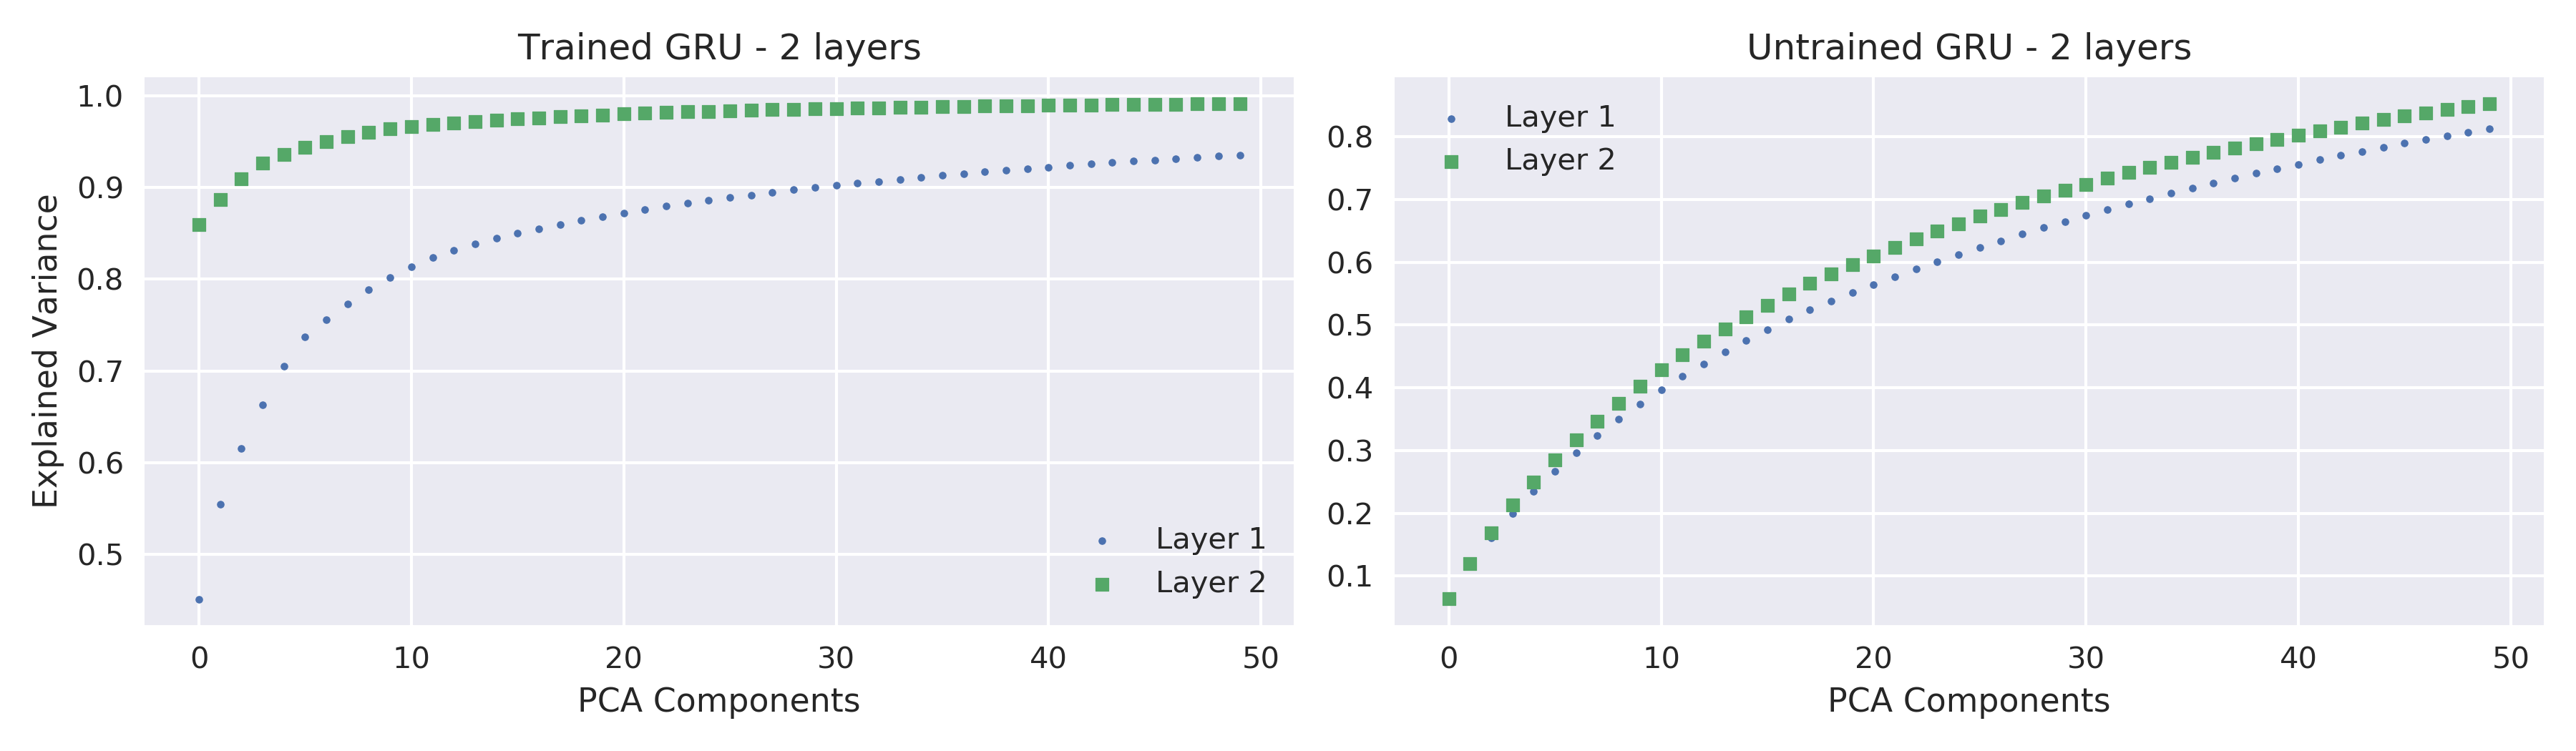
\includegraphics[width=\textwidth]{../images/gru_2layer_100_explained_variance.png}
  \caption{2 layers GRU explained variance}
  \label{fig:-images-gru_2layer_explained_variance-png}
\end{figure}
\begin{figure}[H]
  \centering
  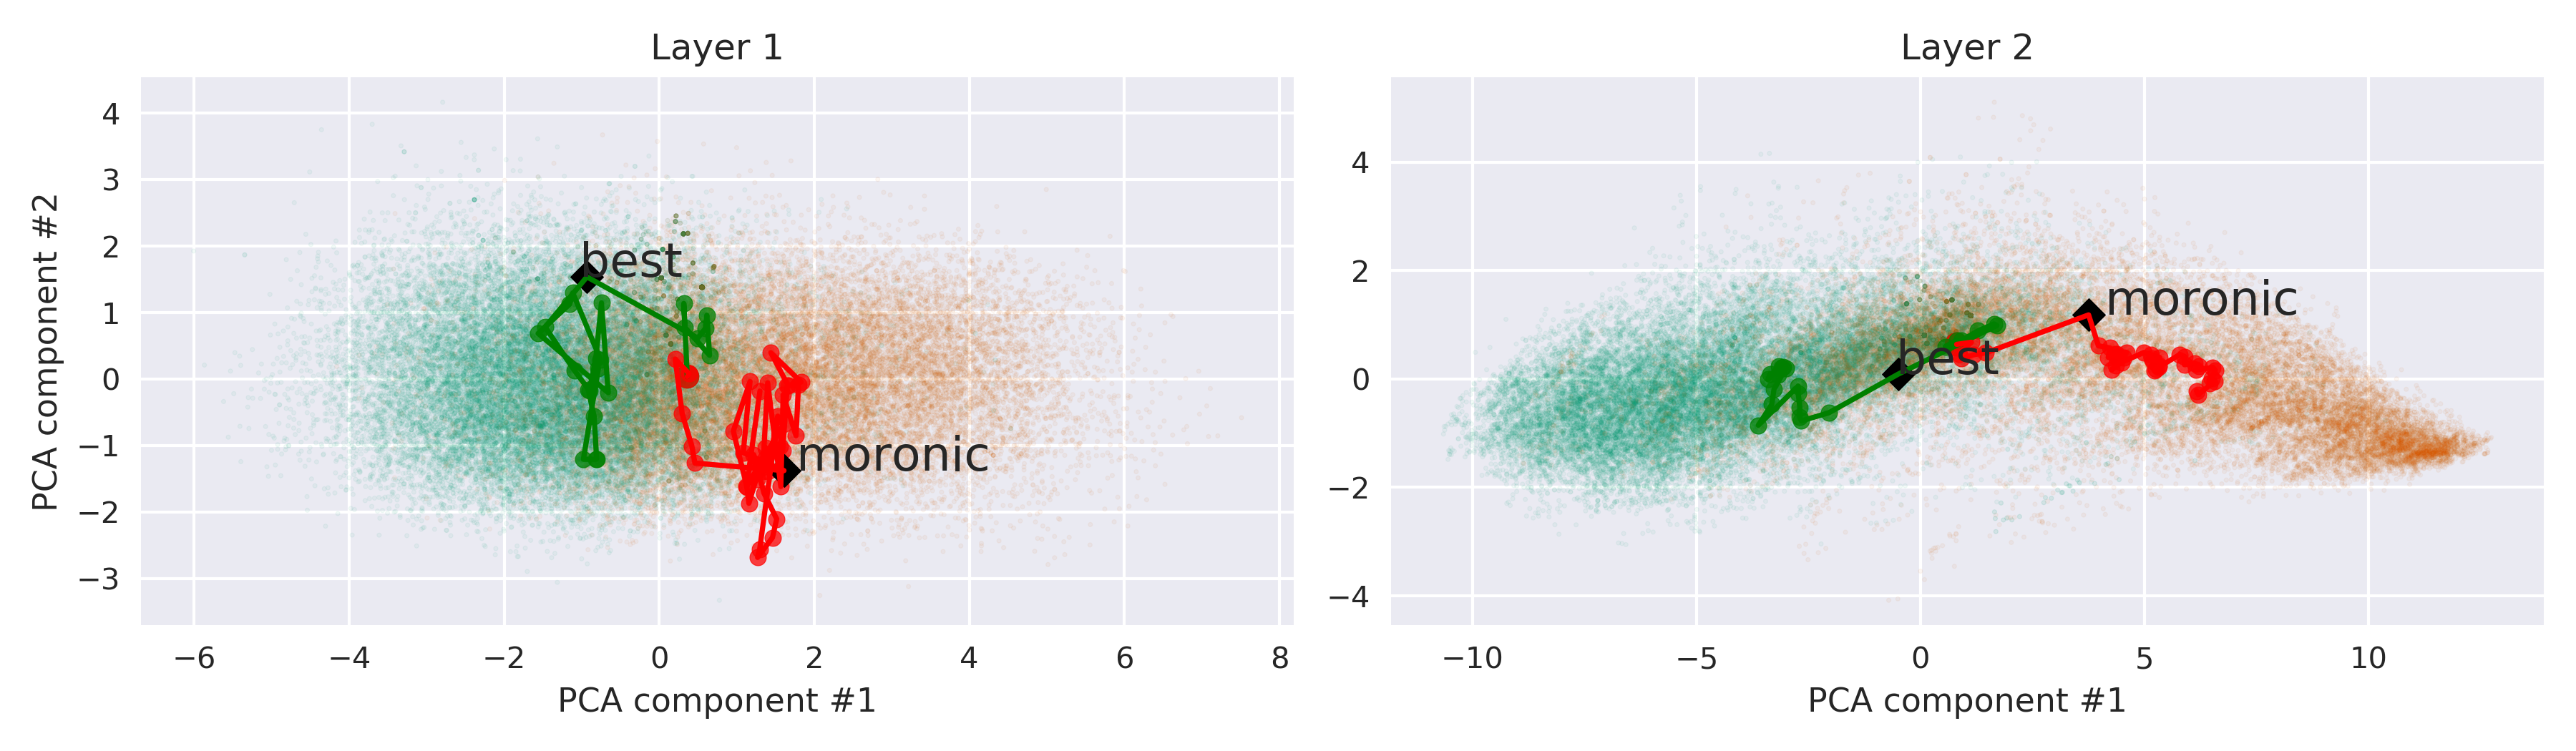
\includegraphics[width=\textwidth]{../images/gru_2layer_100_PCA.png}
  \caption{2 layers GRU PCA}
  \label{fig:-images-gru_2layer_PCA-png}
\end{figure}
\begin{figure}[H]
  \centering
  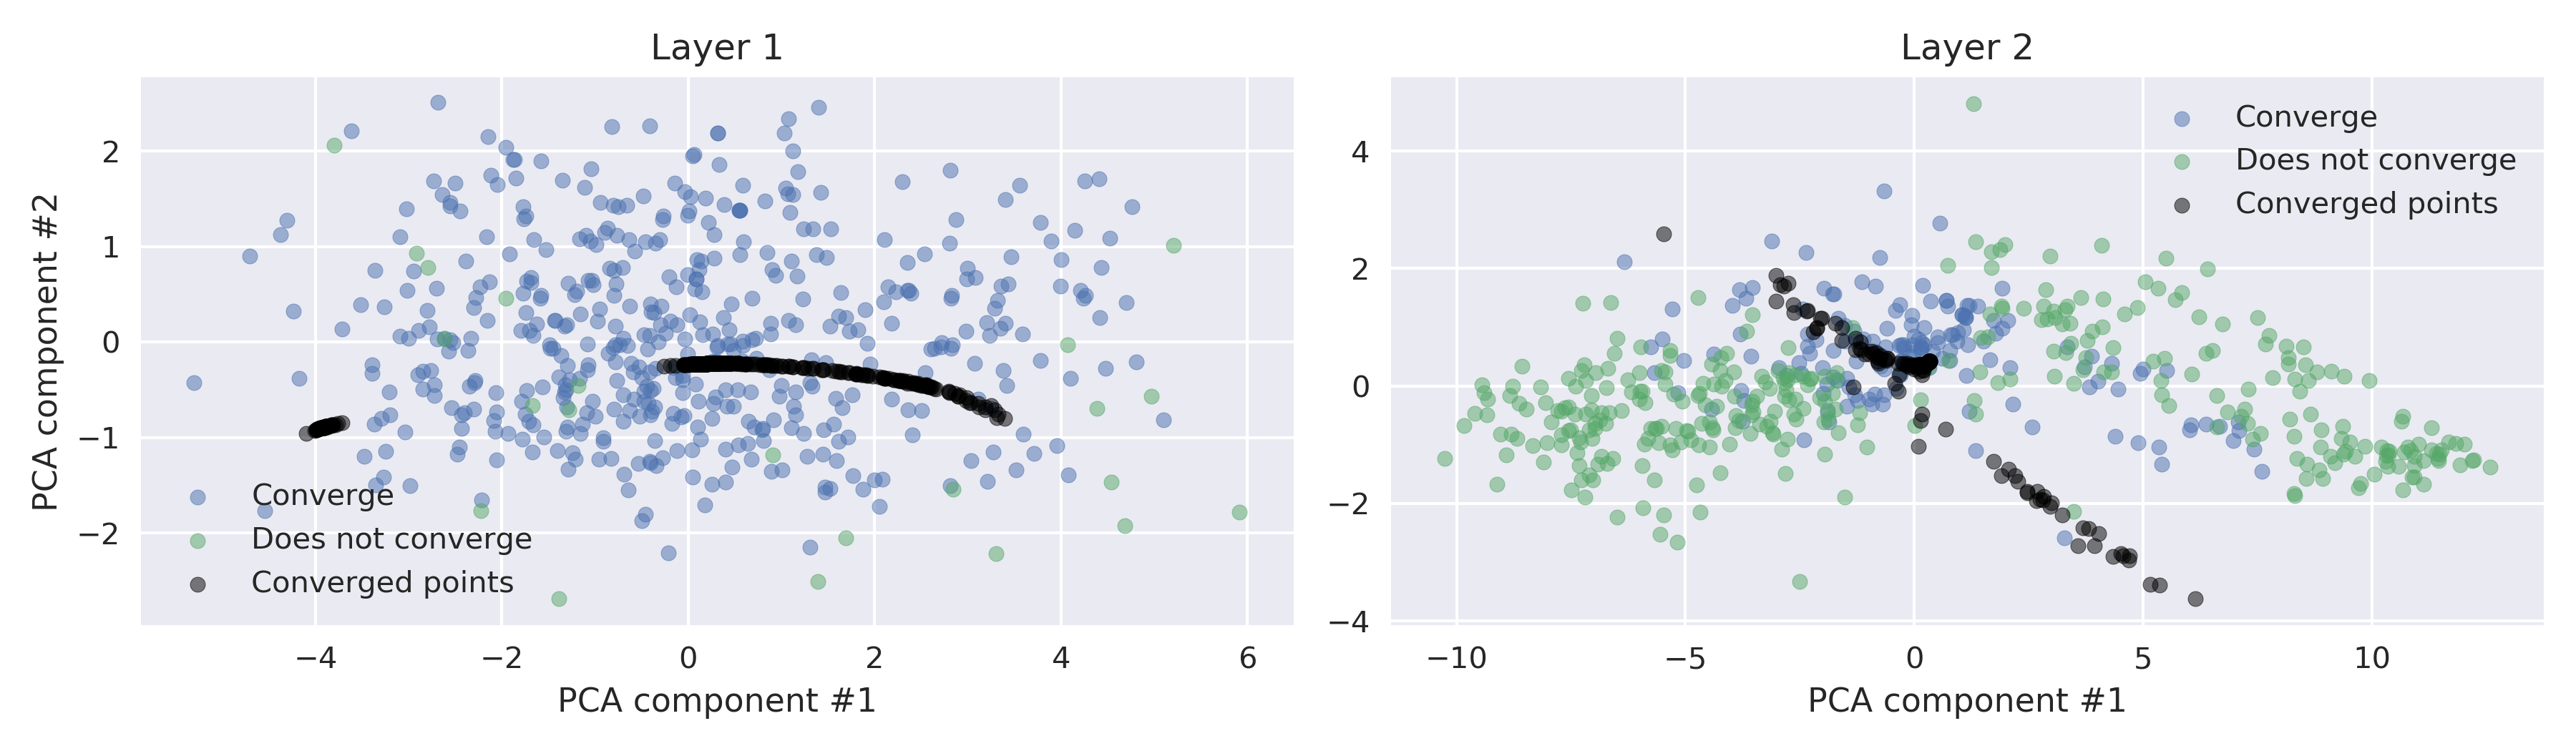
\includegraphics[width=\textwidth]{../images/gru_2layer_100_fixed_points.png}
  \caption{2 layers GRU fixed points}
  \label{fig:-images-gru_2layer_fixed_points-png}
\end{figure}
\begin{figure}[H]
  \centering
  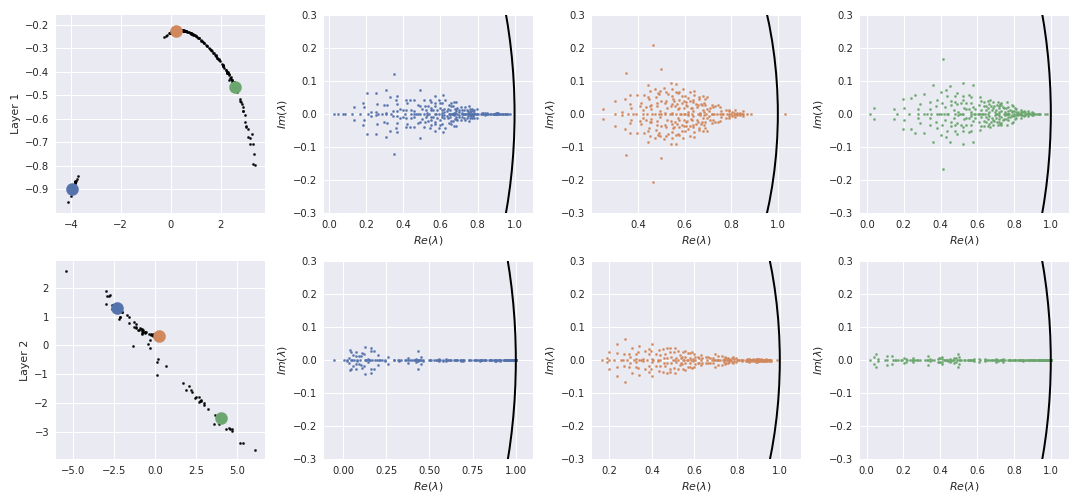
\includegraphics[width=\textwidth]{../images/gru_2layer_100_eig.png}
  \caption{2 layers GRU eigenvalues}
  \label{fig:-images-gru_2layer_eig-png}
\end{figure}

\subsection{3 layers - Embedding of 50 dimension}
\label{anx:3-layers-50}
\begin{figure}[H]
  \centering
  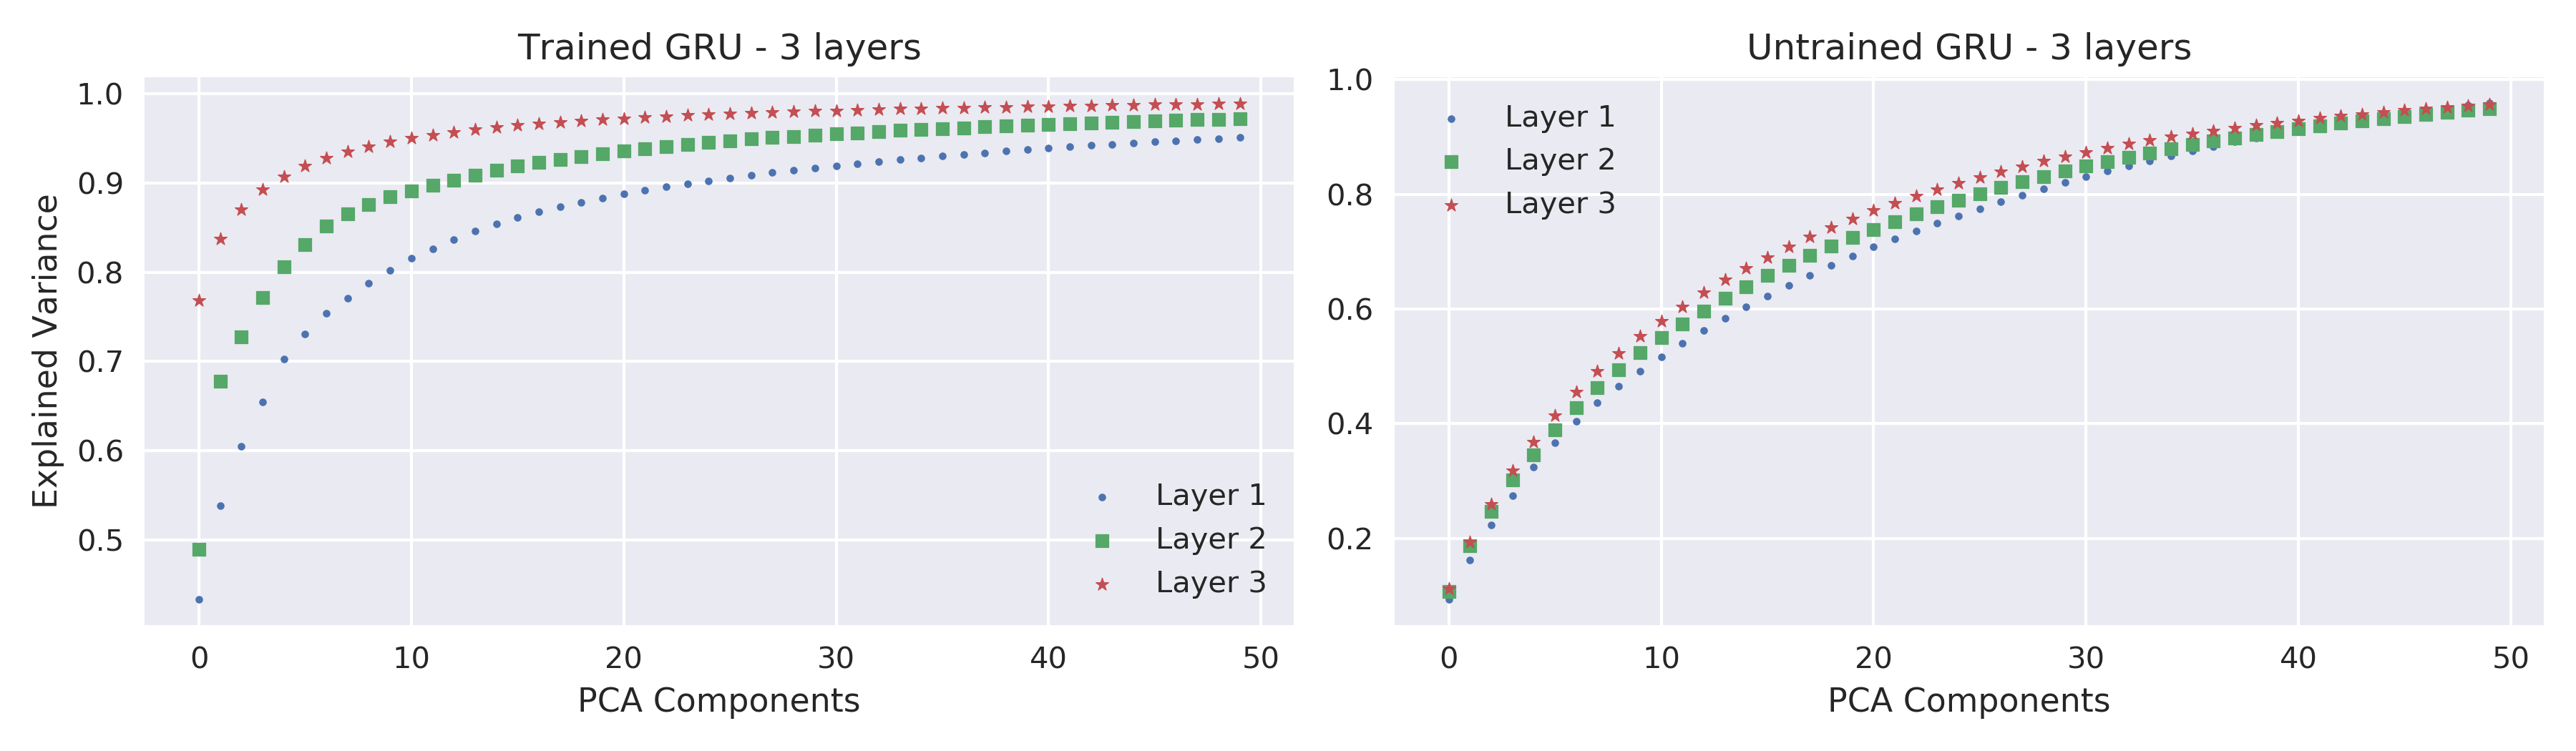
\includegraphics[width=\textwidth]{../images/gru_3layer_50_explained_variance.png}
  \caption{3 layers GRU explained variance}
  \label{fig:-images-gru_3layer_50_explained_variance-png}
\end{figure}
\begin{figure}[H]
  \centering
  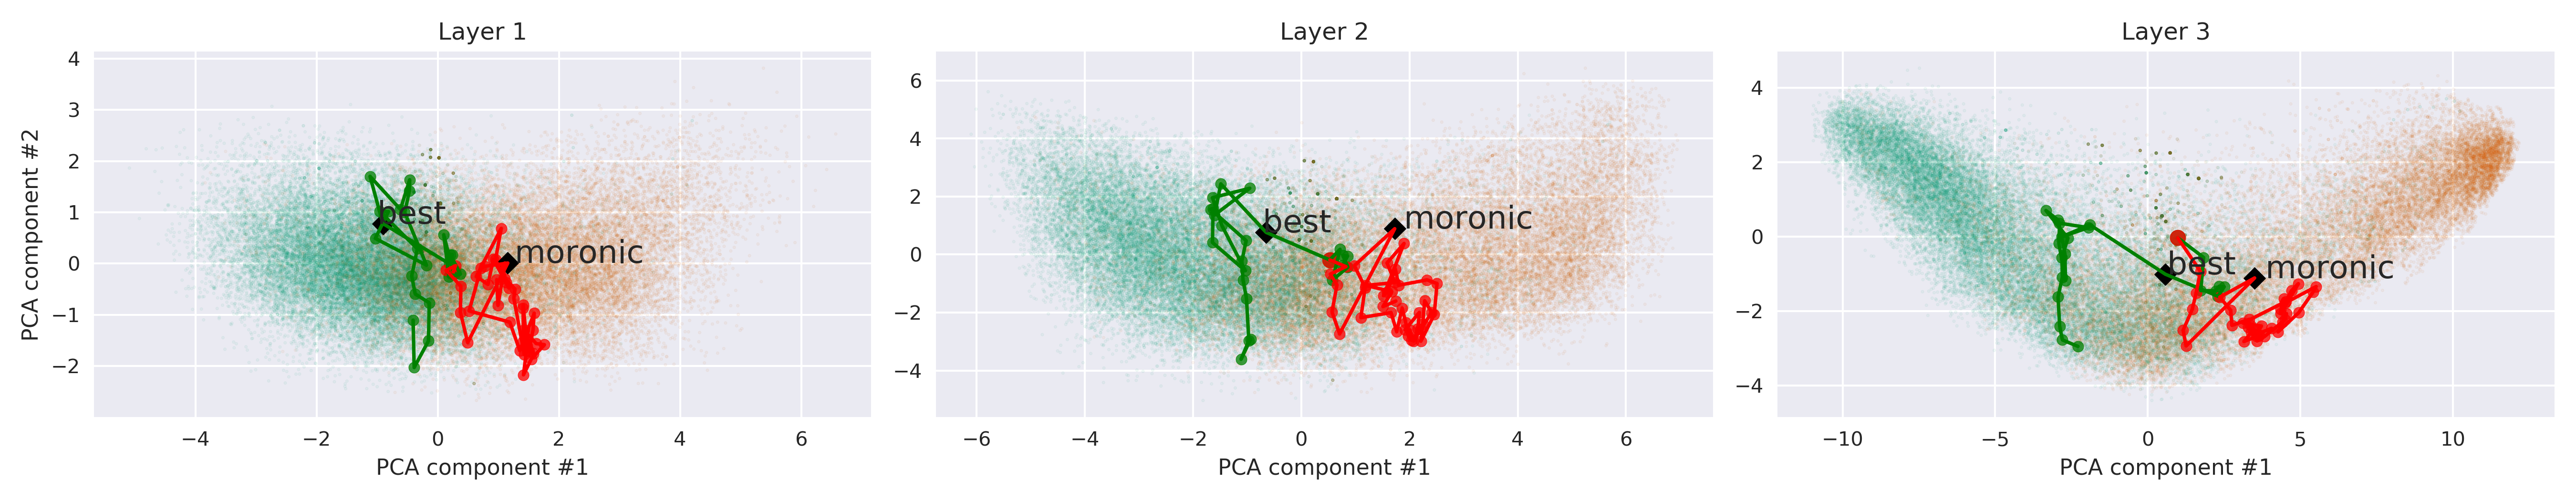
\includegraphics[width=\textwidth]{../images/gru_3layer_50_PCA.png}
  \caption{3 layers GRU PCA}
  \label{fig:-images-gru_3layer_50_PCA-png}
\end{figure}
\begin{figure}[H]
  \centering
  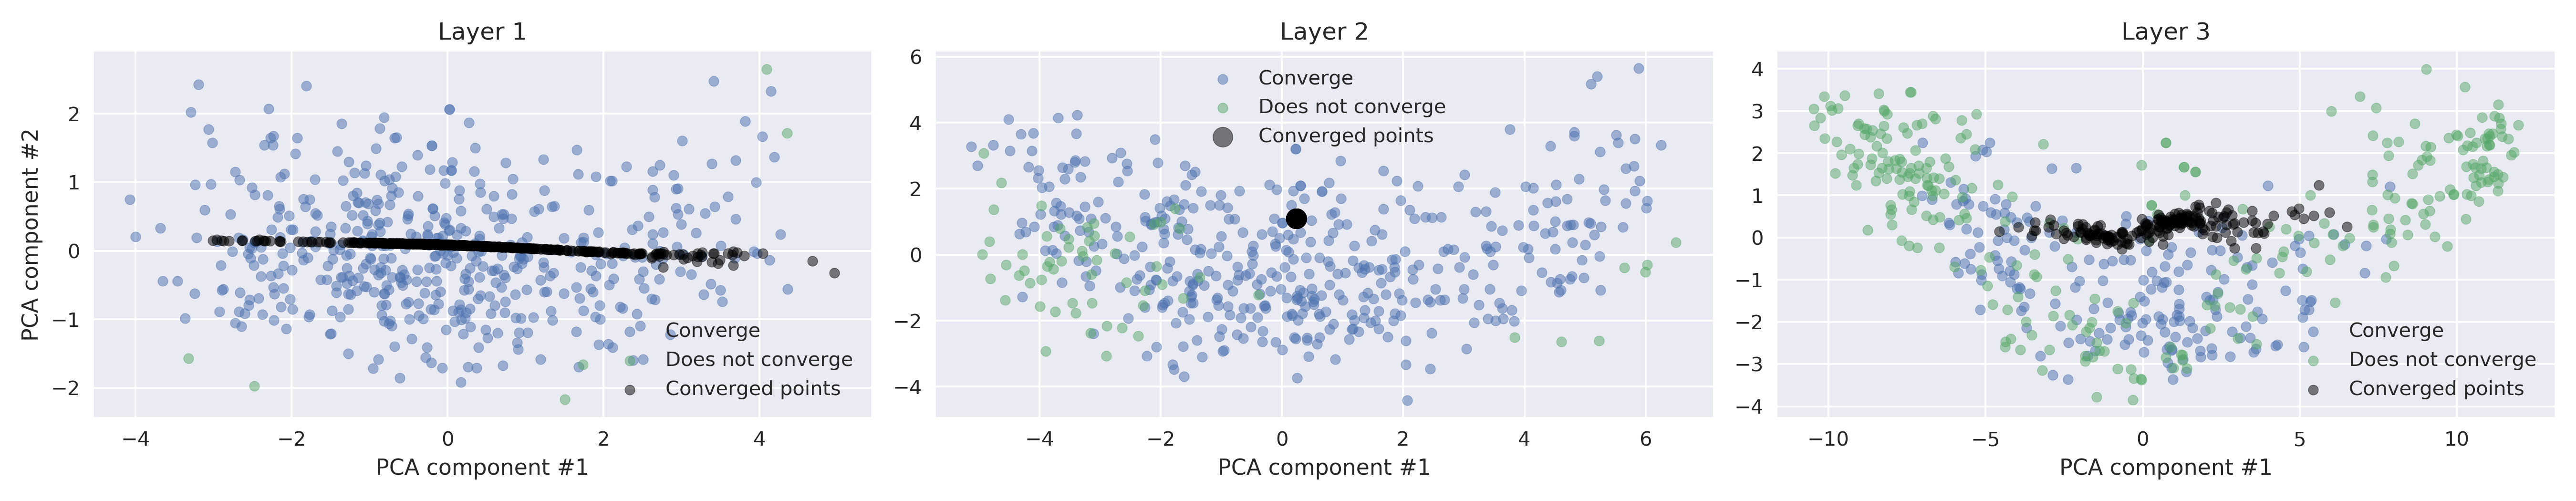
\includegraphics[width=\textwidth]{../images/gru_3layer_50_fixed_points.png}
  \caption{3 layers GRU fixed points}
  \label{fig:-images-gru_3layer_50_fixed_points-png}
\end{figure}
\begin{figure}[H]
  \centering
  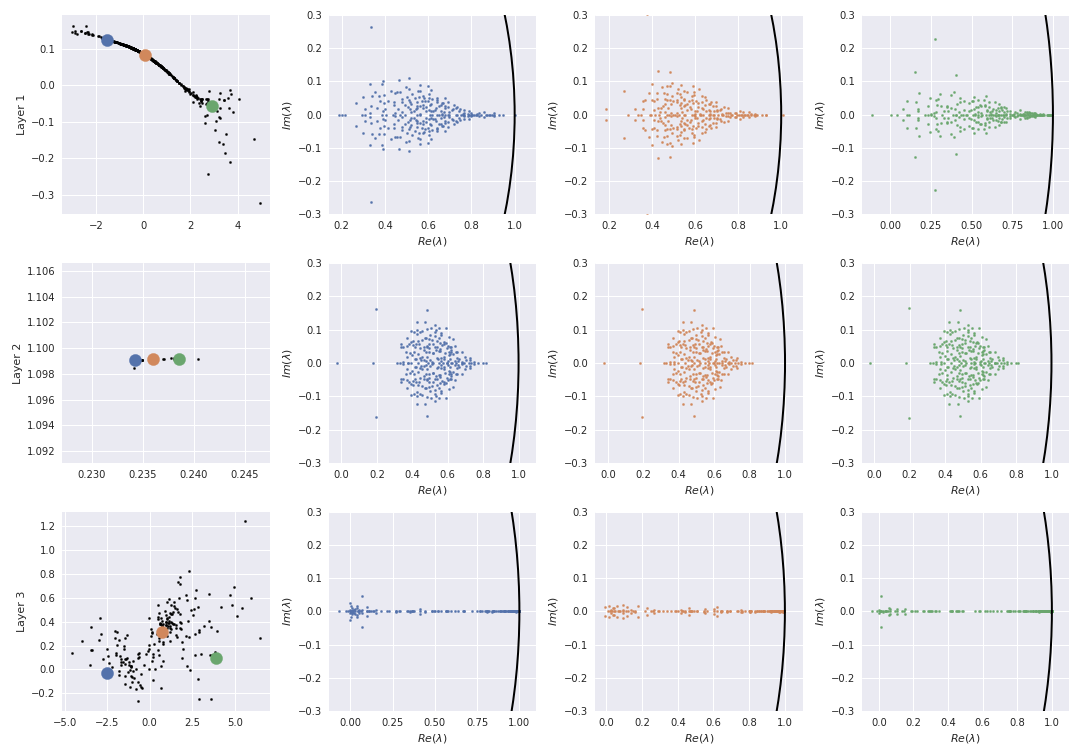
\includegraphics[width=\textwidth]{../images/gru_3layer_50_eig.png}
  \caption{3 layers GRU eigenvalues}
  \label{fig:-images-gru_3layer_50_eig-png}
\end{figure}
\subsection{4 layers}
\label{anx:4-layers}
\begin{figure}[H]
  \centering
  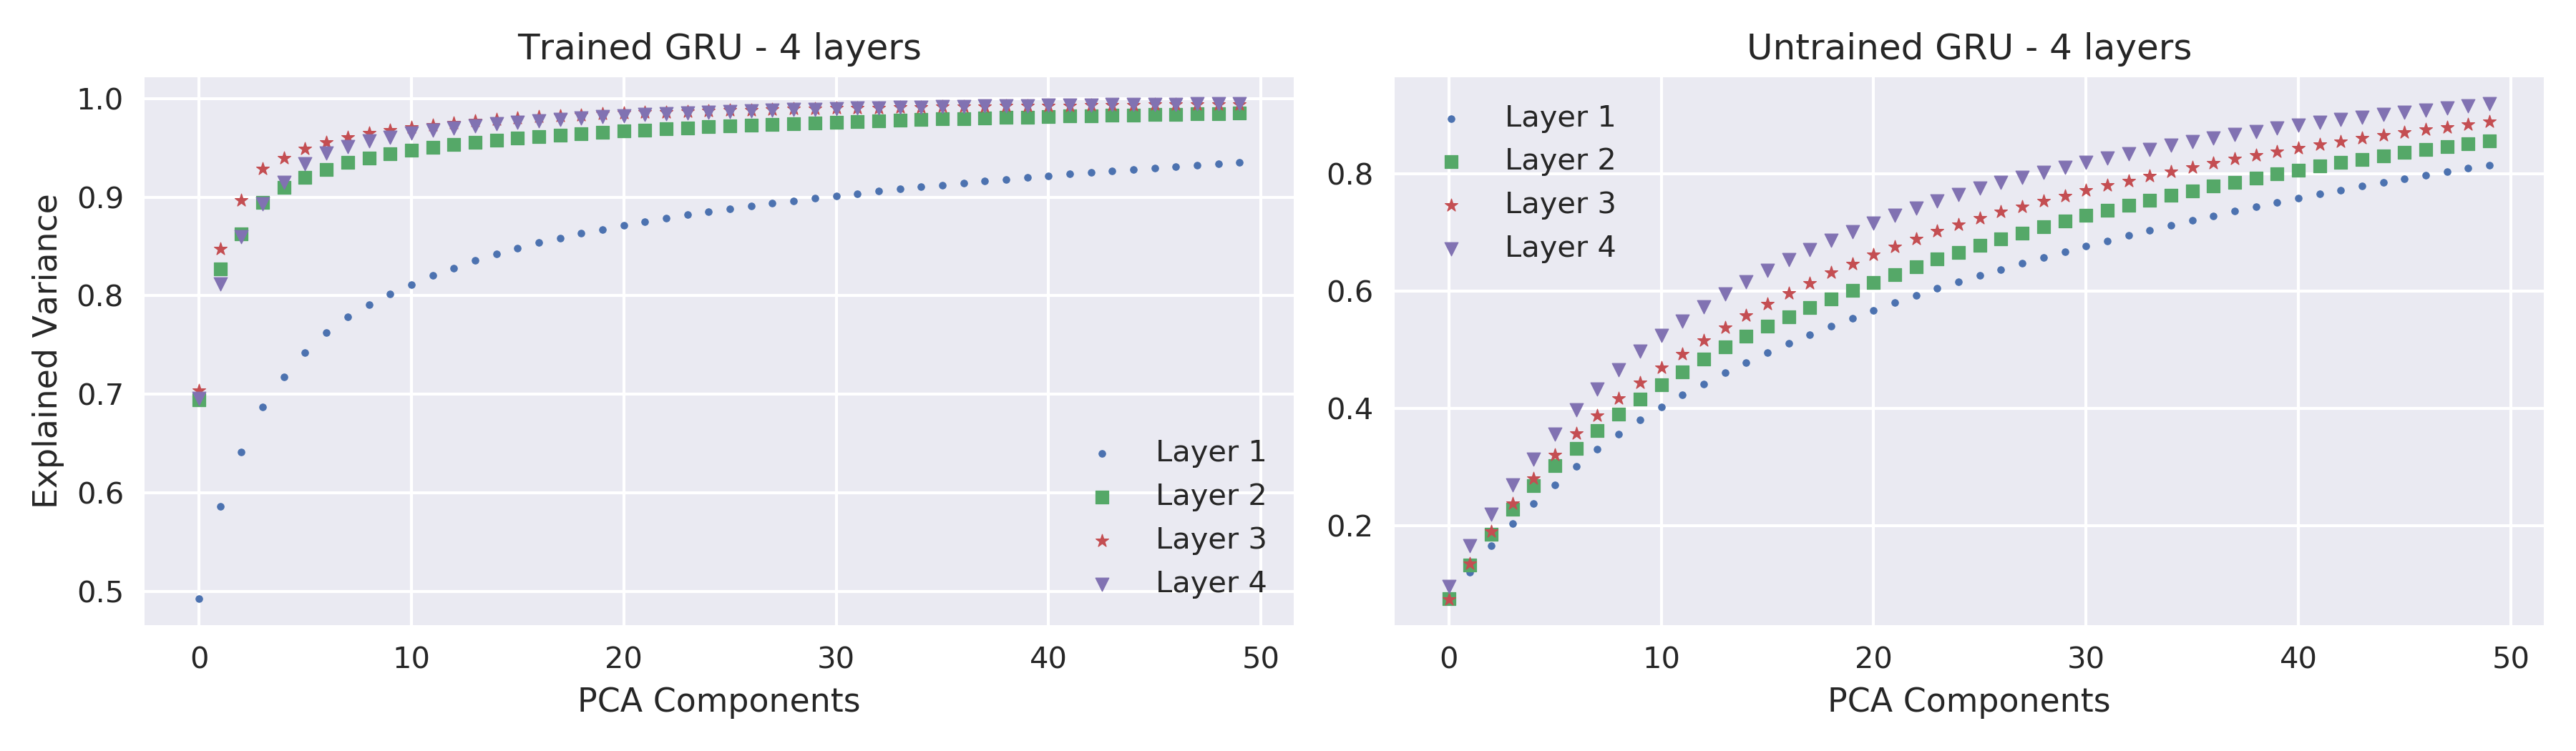
\includegraphics[width=\textwidth]{../images/gru_4layer_100_explained_variance.png}
  \caption{4 layers GRU explained variance}
  \label{fig:-images-gru_4layer_explained_variance-png}
\end{figure}
\begin{figure}[H]
  \centering
  \includegraphics[width=\textwidth]{../images/gru_4layer_100_PCA.png}
  \caption{4 layers GRU PCA}
  \label{fig:-images-gru_4layer_PCA-png}
\end{figure}
\begin{figure}[H]
  \centering
  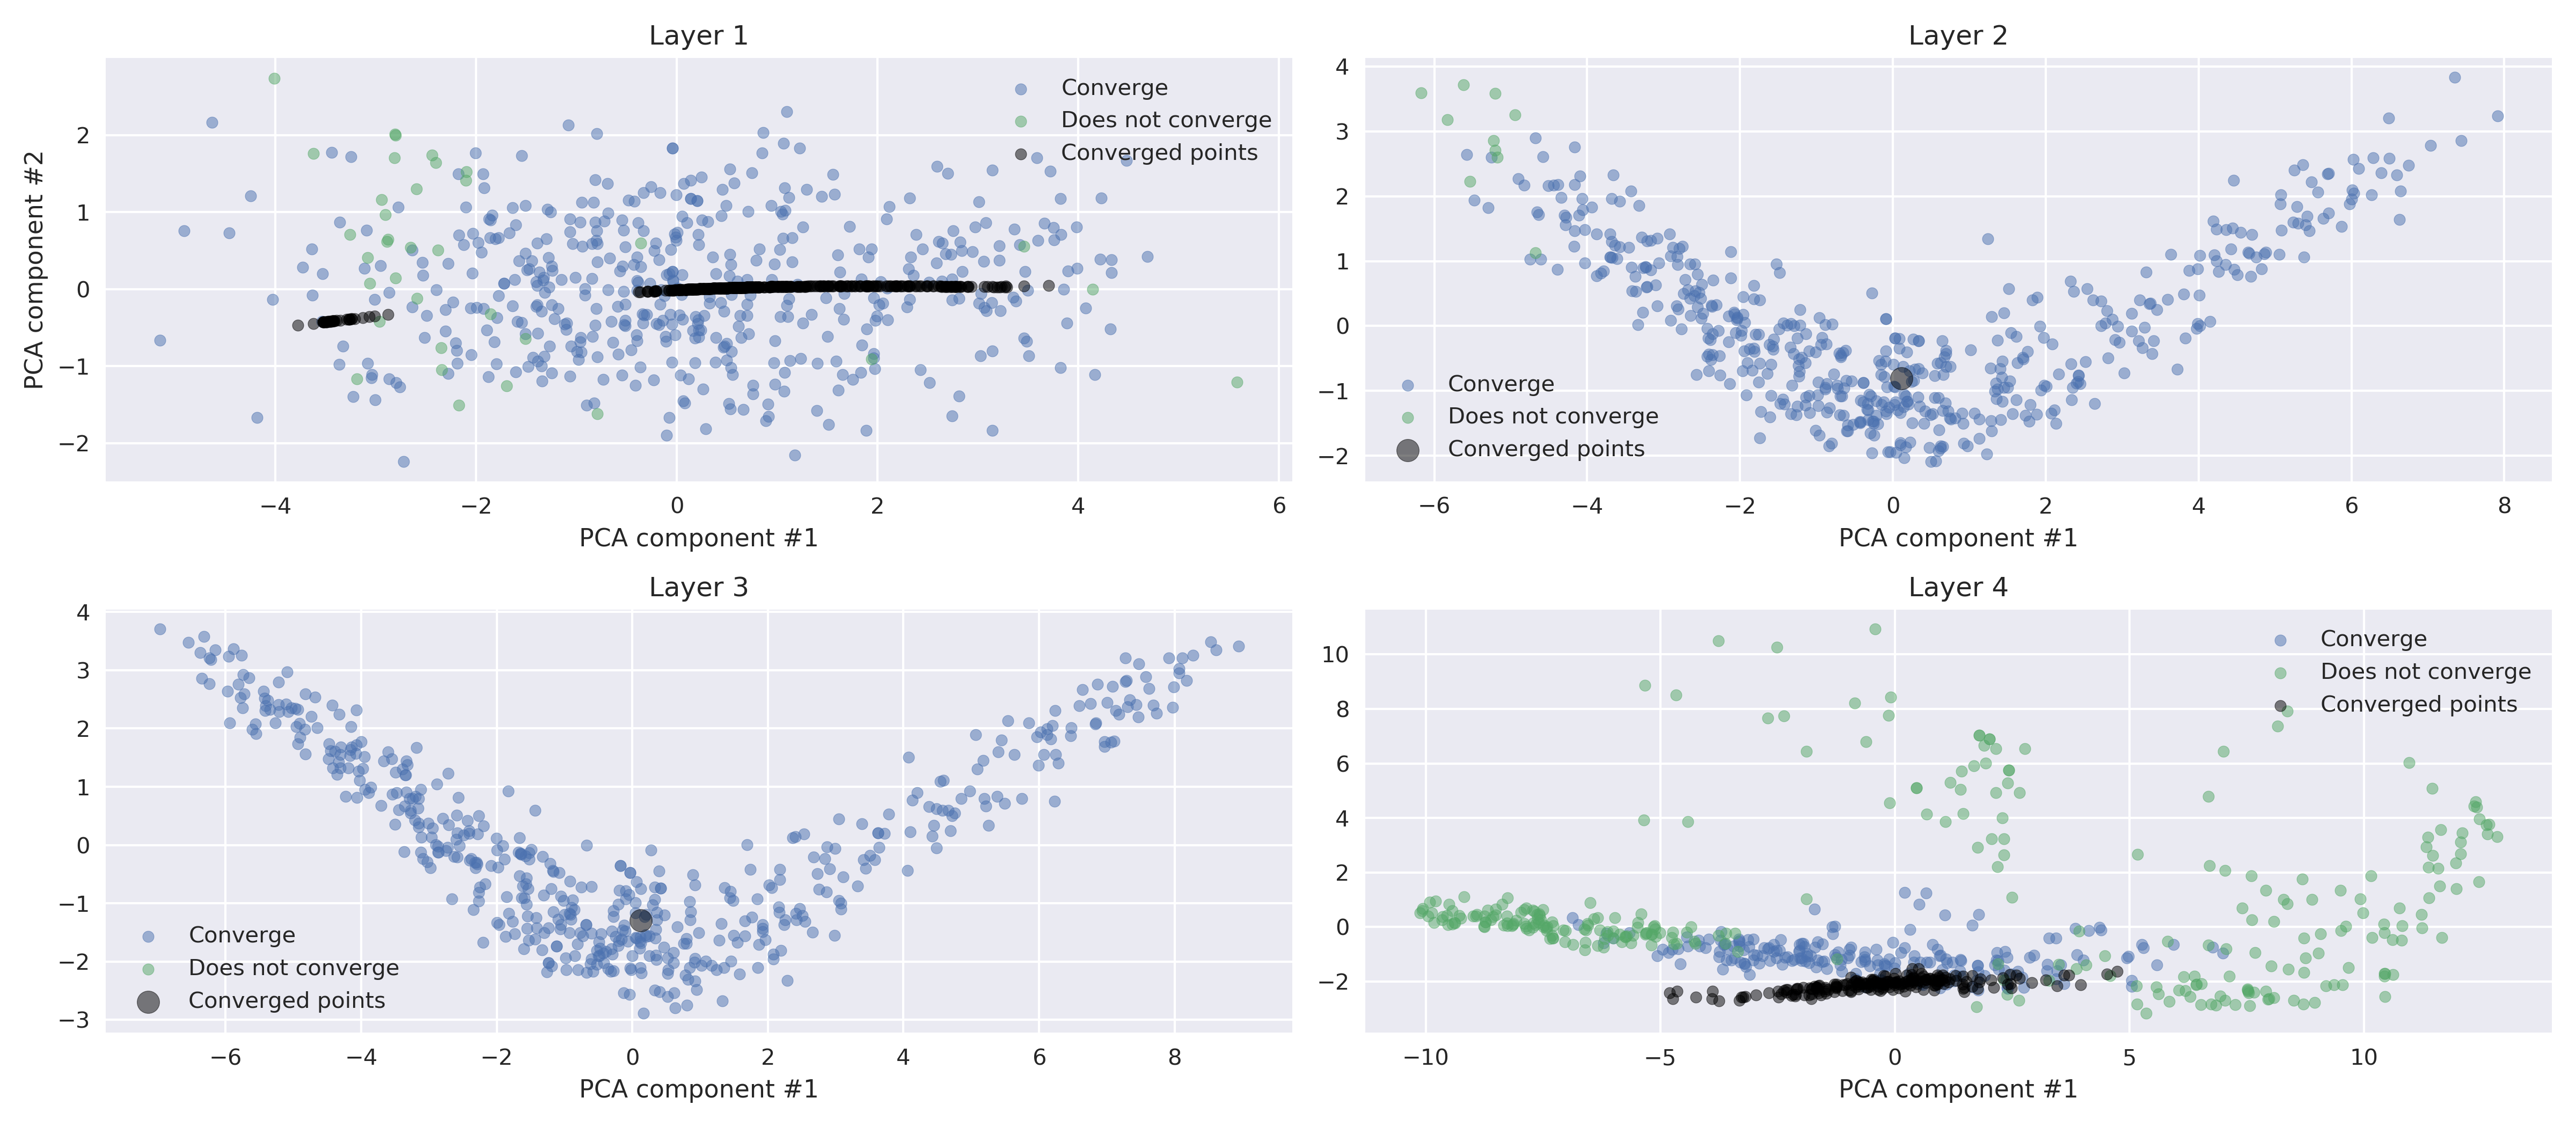
\includegraphics[width=\textwidth]{../images/gru_4layer_100_fixed_points.png}
  \caption{4 layers GRU fixed points}
  \label{fig:-images-gru_4layer_fixed_points-png}
\end{figure}
\begin{figure}[H]
  \centering
  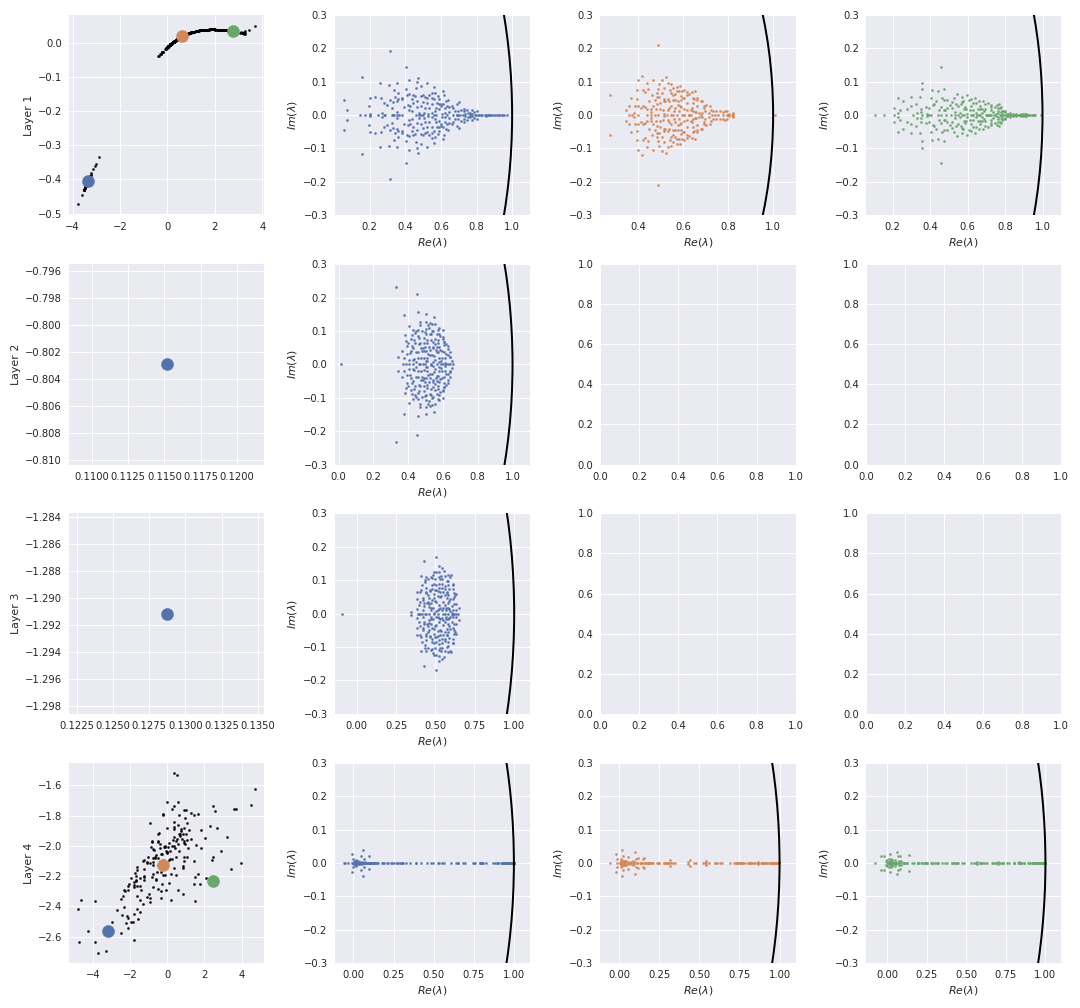
\includegraphics[width=\textwidth]{../images/gru_4layer_100_eig.png}
  \caption{4 layers GRU eigenvalues}
  \label{fig:-images-gru_4layer_eig-png}
\end{figure}
%}}}1
\small


\bibliographystyle{plain}
\bibliography{mat6115.bib}

\end{document}
